%%%%%%%%%%%%%%%%%%%%%%%%%%%%%%
%%%%%%%%%%%%%%%%%%%%%%%%%%%%%%

% To use this template, copy and paste the Template folder found here an place within the folder your beamer presentation is located.
% Make sure to include the following code as the first two lines of your document:
% \documentclass[compress]{beamer}
% \ProvidesPackageRCS $Header: SDAL_Beamer.sty ,v 1 05/13/2016 $

\mode<presentation>

% Set presentation size

\usepackage[orientation=landscape,size=custom,width=16,height=9,scale=0.5,debug]{beamerposter} 
\setbeamersize{text margin left=.25in,text margin right=.25in}

% Set Fonts

%\usepackage[T1]{fontenc}
%\usepackage[default]{raleway}
 
 \usefonttheme{serif}
 
 \setbeamerfont{frametitle}{series=\bfseries} 
\setbeamerfont{title}{series=\bfseries} 
\setbeamerfont{author}{series=\bfseries} 

%\usepackage[T1]{fontenc}
%\usepackage[nosfdefault]{raleway}

% Set the size of the font

\usepackage{scrextend}
\changefontsizes{14pt}
\setbeamerfont{title}{size=\fontsize{17pt}{17pt}}
\setbeamerfont{author}{size=\fontsize{14pt}{14pt}}
\setbeamerfont{frametitle}{size=\fontsize{17pt}{17pt}}
\setbeamerfont{date}{size=\fontsize{14pt}{14pt}}
\setbeamerfont*{structure}{size*={17pt}{17pt}}
\setbeamerfont*{tiny structure}{size*={6pt}{6pt}}
  
% Table of Contents

\setbeamertemplate{section in toc}[ball]
\setbeamertemplate{subsection in toc}[square]

\setbeamertemplate{subsection in toc}{\hspace{1.2em}{\color{BIlightblue}\rule[0.3ex]{6pt}{6pt}}~\inserttocsubsection\par}

% Set Color

\definecolor{VTmaroon}{RGB}{102,0,0} 
\definecolor{VTorange}{RGB}{255,102,0}
\definecolor{BIdarkblue}{RGB}{18,37,45}
\definecolor{BIaquablue}{RGB}{126,168,173}
\definecolor{BIcoolgrey}{RGB}{153,153,153}
\definecolor{BIlightblue}{RGB}{93,137,180}
\definecolor{BIlightgreen}{RGB}{141,194,136}

 
\setbeamercolor*{title}{fg=black}
\setbeamercolor{author}{fg=black} 
\setbeamercolor{frametitle}{fg=black} 
\setbeamercolor{section in toc}{fg=black}
\setbeamercolor{subsection in toc}{fg=black}
\setbeamercolor{itemize subsubitem}{fg=black}
\setbeamercolor{itemize subitem}{fg=black}
\setbeamercolor{itemize item}{fg=black}
\setbeamercolor{section number projected}{bg=BIlightblue,fg=white}

% Lists

\makeatletter
\renewcommand{\itemize}[1][]{%
  \beamer@ifempty{#1}{}{\def\beamer@defaultospec{#1}}%
  \ifnum \@itemdepth >2\relax\@toodeep\else
    \advance\@itemdepth\@ne
    \beamer@computepref\@itemdepth% sets \beameritemnestingprefix
    \usebeamerfont{itemize/enumerate \beameritemnestingprefix body}%
    \usebeamercolor[fg]{itemize/enumerate \beameritemnestingprefix body}%
    \usebeamertemplate{itemize/enumerate \beameritemnestingprefix body begin}%
    \list
      {\usebeamertemplate{itemize \beameritemnestingprefix item}}
      {%
        \setlength\topsep{0pt}%NEW
        \setlength\partopsep{0pt}%NEW
        \setlength\itemsep{0pt}%NEW
        \def\makelabel##1{%
          {%
            \hss\llap{{%
                \usebeamerfont*{itemize \beameritemnestingprefix item}%
                \usebeamercolor[fg]{itemize \beameritemnestingprefix item}##1}}%
          }%
        }%
      }
  \fi%
  \beamer@cramped%
  \raggedright%
  \beamer@firstlineitemizeunskip%
}
\makeatother

\setlength\topsep{-10pt}
\setlength\partopsep{-10pt}


\setbeamertemplate{itemize items}[circle]
\setbeamertemplate{itemize subitem}{---}
\setbeamertemplate{itemize subsubitem}[circle]

% TOC

\makeatletter
\patchcmd{\beamer@sectionintoc}
  {\vfill}
  {\vskip\itemsep}
  {}
  {}
\makeatother  

% Remove navigation symbols

\setbeamertemplate{navigation symbols}{}

% Format Title Page

\defbeamertemplate*{title page}{customized}[1][]
{
\centering
\vspace{.9in}\hspace*{-3.8in}
\begin{overlayarea}{4.1in}{1cm}
\centering{
\usebeamerfont{title}\inserttitle\par}
\usebeamerfont{subtitle}\usebeamercolor[fg]{subtitle}\insertsubtitle\par
\end{overlayarea}\\
\vspace{.2in}\hspace*{-1in}
\begin{overlayarea}{4in}{1cm}
\centering{
\usebeamerfont{date}\insertdate\par \vspace{.1in}
\usebeamerfont{author}\insertauthor\par
\usebeamerfont{institute}\insertinstitute\par}
\end{overlayarea}
}

%%% Formatting Different Frame Styles

% Title

\makeatletter
\define@key{beamerframe}{Title}[true]{%
\usebackgroundtemplate{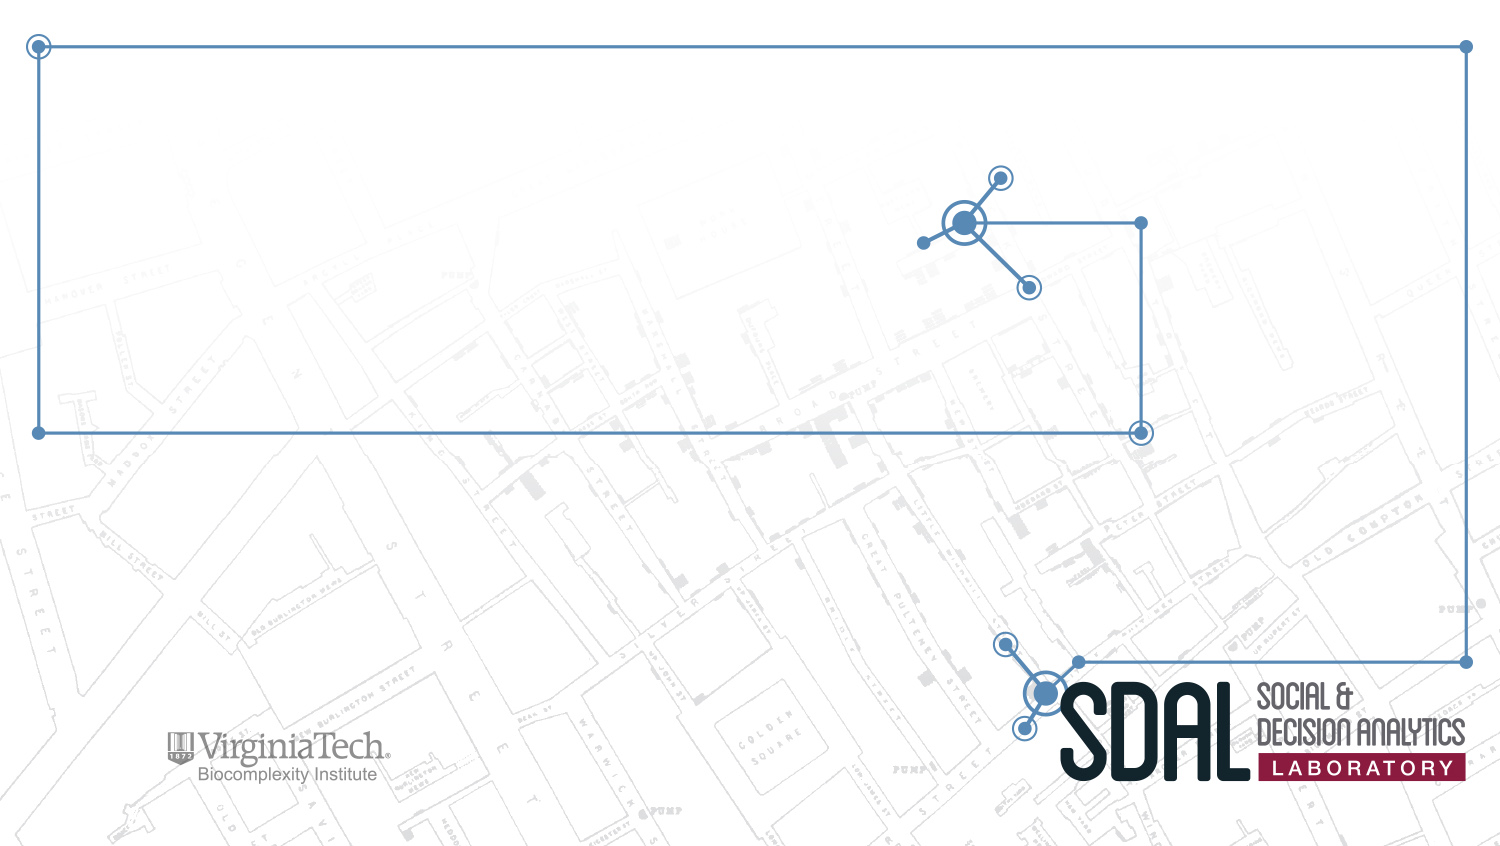
\includegraphics[height=\paperheight,width=\paperwidth]{Template/slides/Title.jpg}
\setbeamertemplate{frametitle}[default][right]
\addtobeamertemplate{frametitle}{\vskip.1in\hspace*{.5in}}{}}
\setbeamertemplate{footline}{}
}
\makeatother

% Outline

\makeatletter
\define@key{beamerframe}{ToC}[true]{%
\usebackgroundtemplate{
\includegraphics[height=\paperheight,width=\paperwidth]{Template/slides/Blank.jpg}}
\setbeamertemplate{frametitle}[default][right]
\addtobeamertemplate{frametitle}{\vskip.1in\hspace*{.5in}}{}
\setbeamertemplate{footline}{}
}
\makeatother

% Blank

\makeatletter
\define@key{beamerframe}{Blank}[true]{%
\usebackgroundtemplate{
\includegraphics[height=\paperheight,width=\paperwidth]{Template/slides/Blank.jpg}}
\setbeamertemplate{frametitle}
{\begin{flushright}\vspace{.23in}{\insertframetitle\hspace{.2in}}\end{flushright}}
\setbeamertemplate{footline}{%
\leavevmode%
  \hbox{%
    \begin{beamercolorbox}[wd=\paperwidth,ht=2.5ex,dp=1.125ex]{palette quaternary}%
    \vspace{.08in}\insertnavigation{\paperwidth}{}{\hskip0pt plus1filll}
    \end{beamercolorbox}%
  }
}
}
\makeatother

% BlankLogo

\makeatletter
\define@key{beamerframe}{BlankLogo}[true]{%
\usebackgroundtemplate{
\includegraphics[height=\paperheight,width=\paperwidth]{Template/slides/BlankLogo.jpg}}
\setbeamertemplate{frametitle}
{\begin{flushright}\vspace{.23in}{\insertframetitle\hspace{.2in}}\end{flushright}}
\setbeamertemplate{footline}{}
}
\makeatother

% Basic1

\makeatletter
\define@key{beamerframe}{Basic1}[true]{%
\usebackgroundtemplate{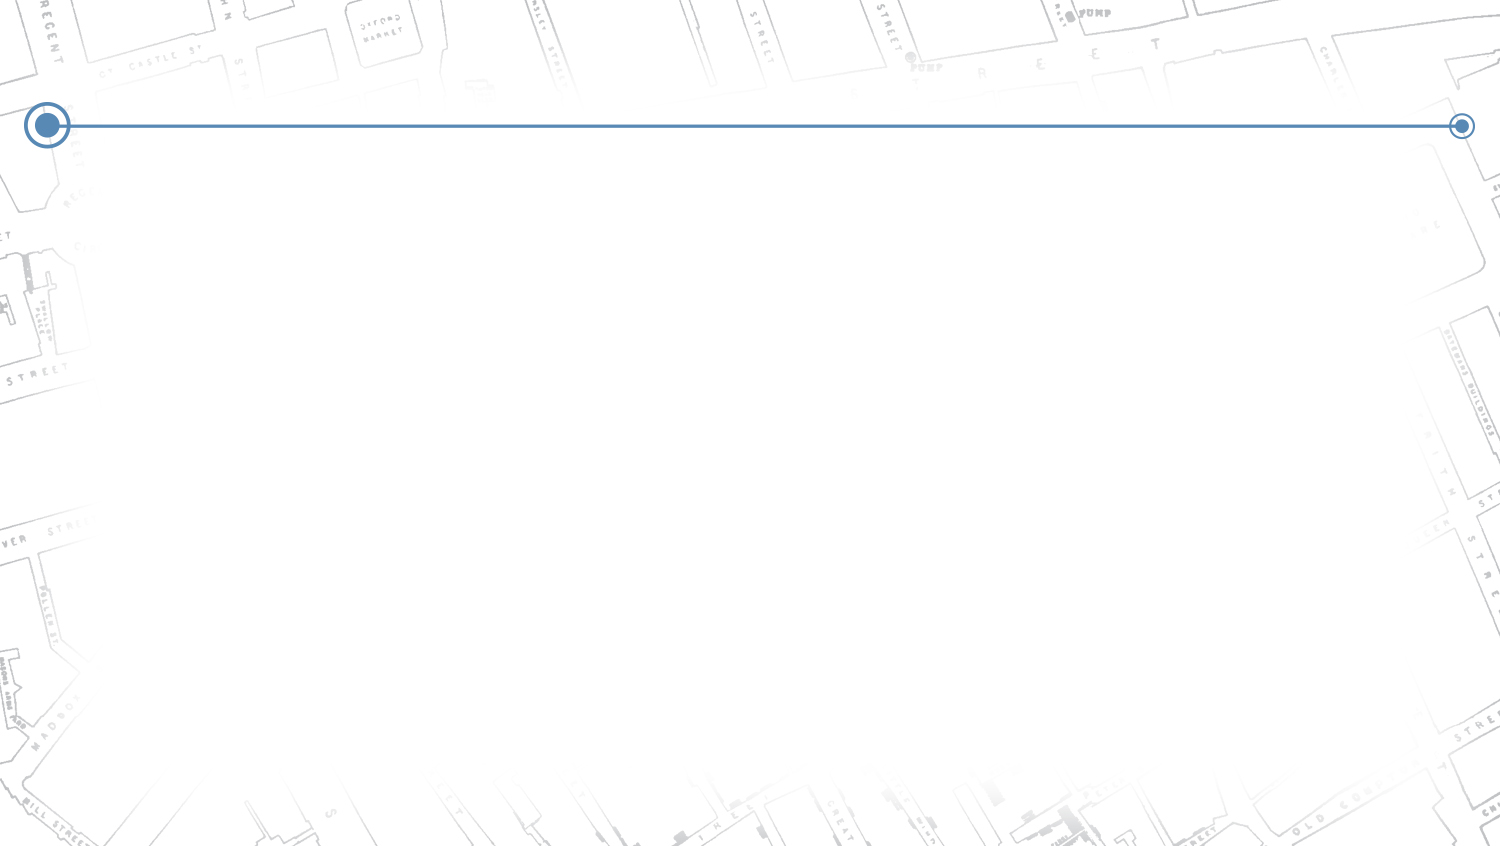
\includegraphics[height=\paperheight,width=\paperwidth]{Template/slides/Basic1.jpg}}
\setbeamertemplate{frametitle}
{\begin{flushright}\vspace{.23in}{\insertframetitle\hspace{.2in}}\end{flushright}}
\setbeamertemplate{footline}{%
\leavevmode%
  \hbox{%
    \begin{beamercolorbox}[wd=\paperwidth,ht=2.5ex,dp=1.125ex]{palette quaternary}%
    \vspace{.08in}\insertnavigation{\paperwidth}{}{\hskip0pt plus1filll}
    \end{beamercolorbox}%
  }
}
}
\makeatother

% Basic2

\makeatletter
\define@key{beamerframe}{Basic2}[true]{%
\usebackgroundtemplate{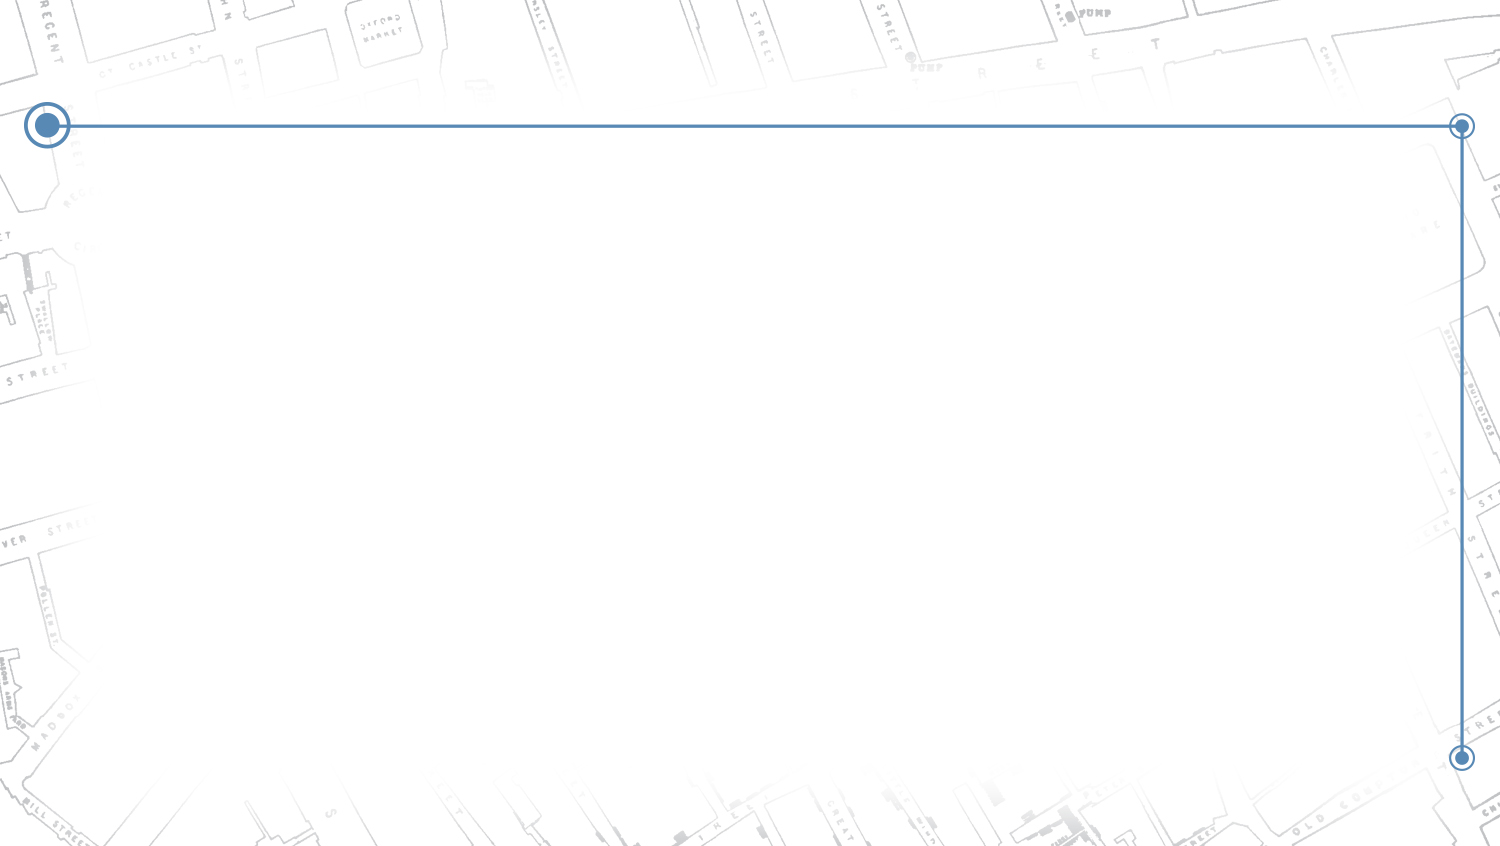
\includegraphics[height=\paperheight,width=\paperwidth]{Template/slides/Basic2.jpg}}
\setbeamertemplate{frametitle}
{\begin{flushright}\vspace{.23in}{\insertframetitle\hspace{.2in}}\end{flushright}}
\setbeamertemplate{footline}{%
\leavevmode%
  \hbox{%
    \begin{beamercolorbox}[wd=\paperwidth,ht=2.5ex,dp=1.125ex]{palette quaternary}%
    \vspace{.08in}\insertnavigation{\paperwidth}{}{\hskip0pt plus1filll}
    \end{beamercolorbox}%
  }
}
}
\makeatother

% Basic3

\makeatletter
\define@key{beamerframe}{Basic3}[true]{%
\usebackgroundtemplate{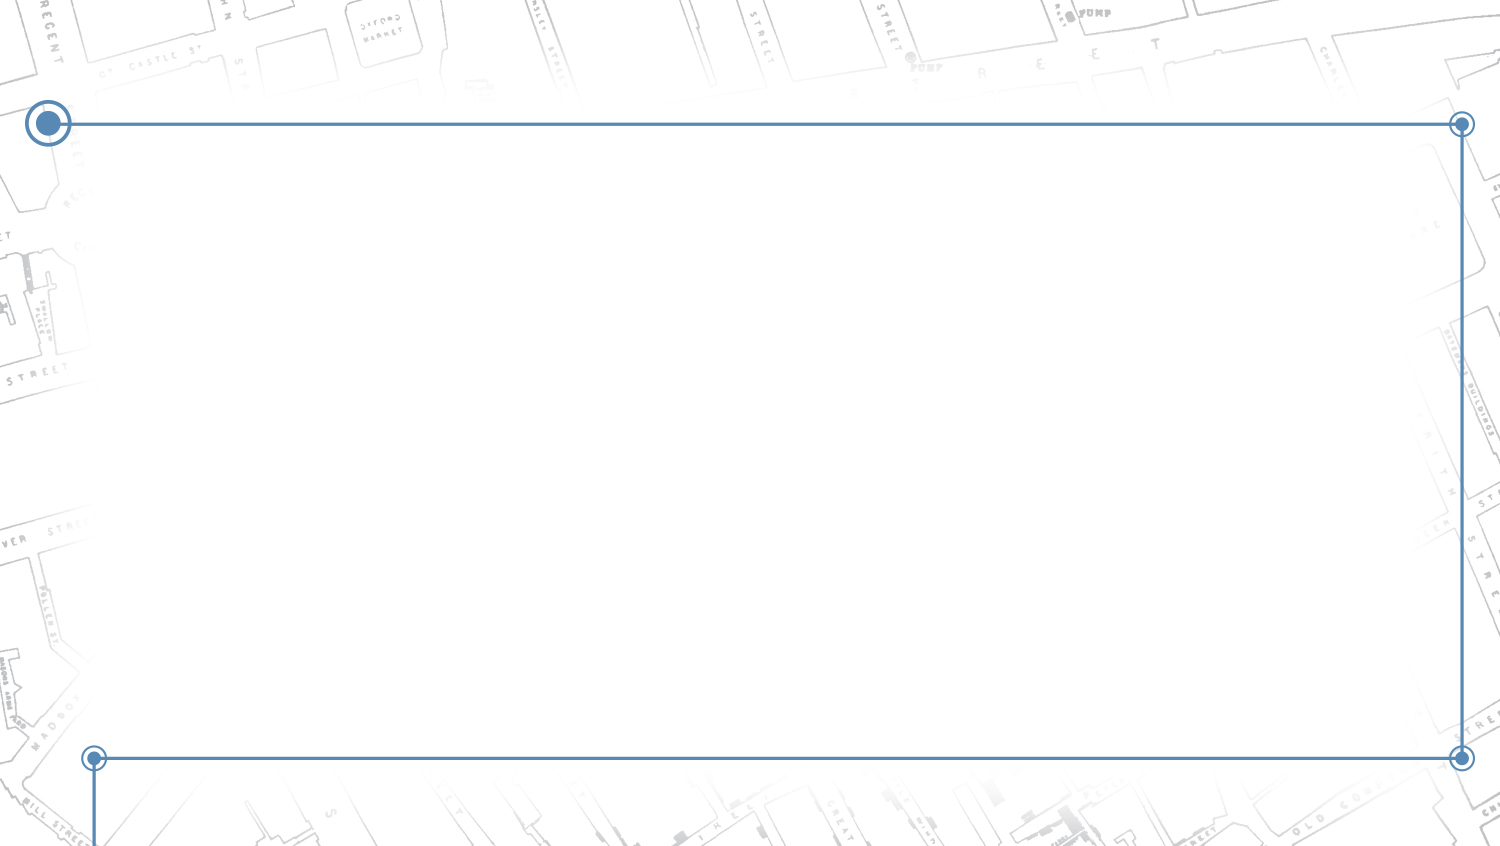
\includegraphics[height=\paperheight,width=\paperwidth]{Template/slides/Basic3.jpg}}
\setbeamertemplate{frametitle}
{\begin{flushright}\vspace{.23in}{\insertframetitle\hspace{.2in}}\end{flushright}}
\setbeamertemplate{footline}{}
}
\makeatother

% Basic1Logo

\makeatletter
\define@key{beamerframe}{Basic1Logo}[true]{%
\usebackgroundtemplate{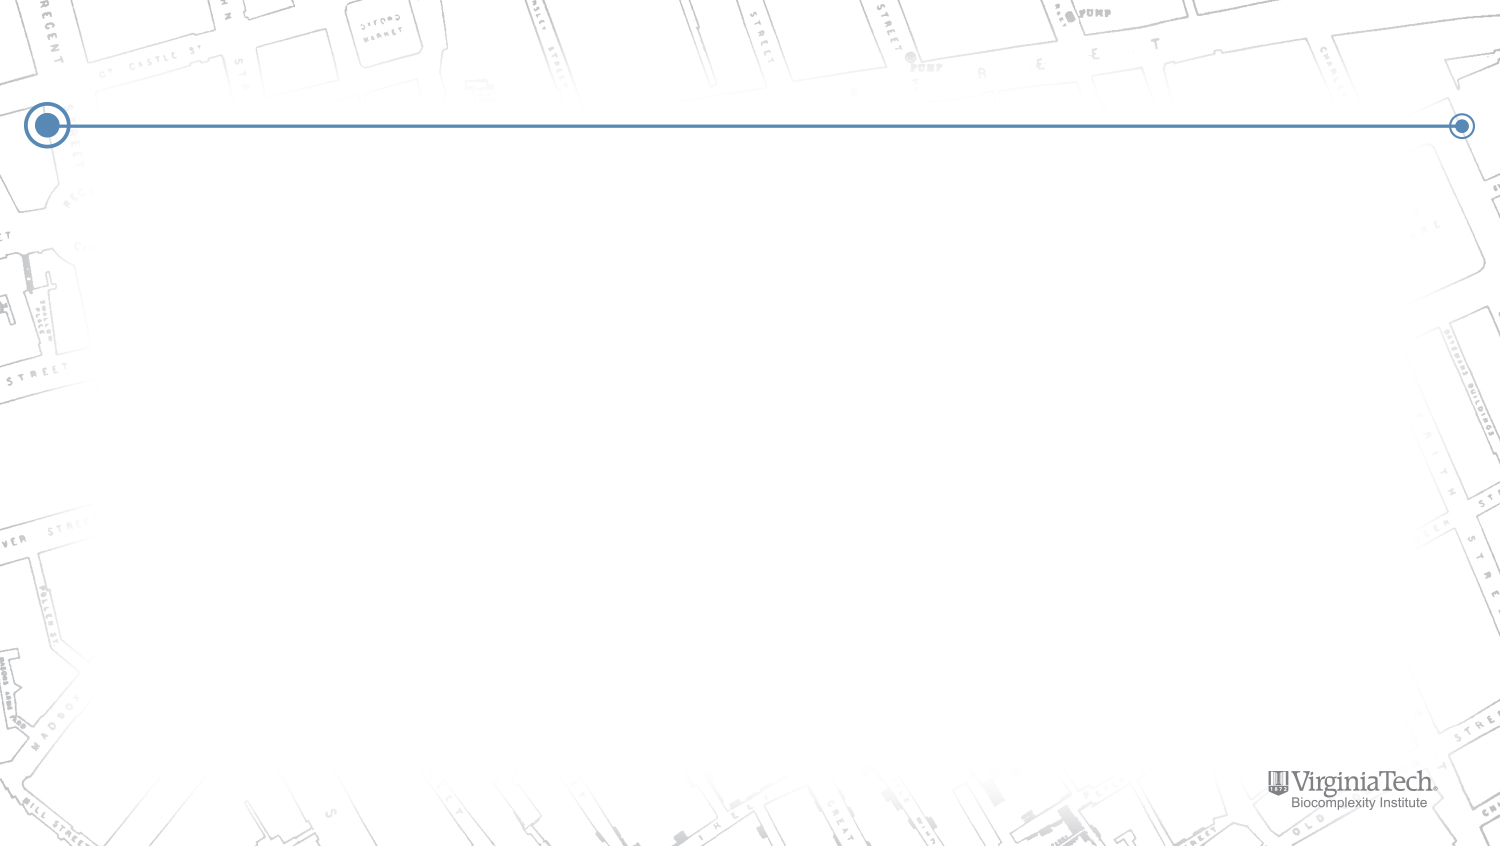
\includegraphics[height=\paperheight,width=\paperwidth]{Template/slides/Basic1Logo.jpg}}
\setbeamertemplate{frametitle}
{\begin{flushright}\vspace{.23in}{\insertframetitle\hspace{.2in}}\end{flushright}}
\setbeamertemplate{footline}{}
}
\makeatother

% Basic2Logo

\makeatletter
\define@key{beamerframe}{Basic2Logo}[true]{%
\usebackgroundtemplate{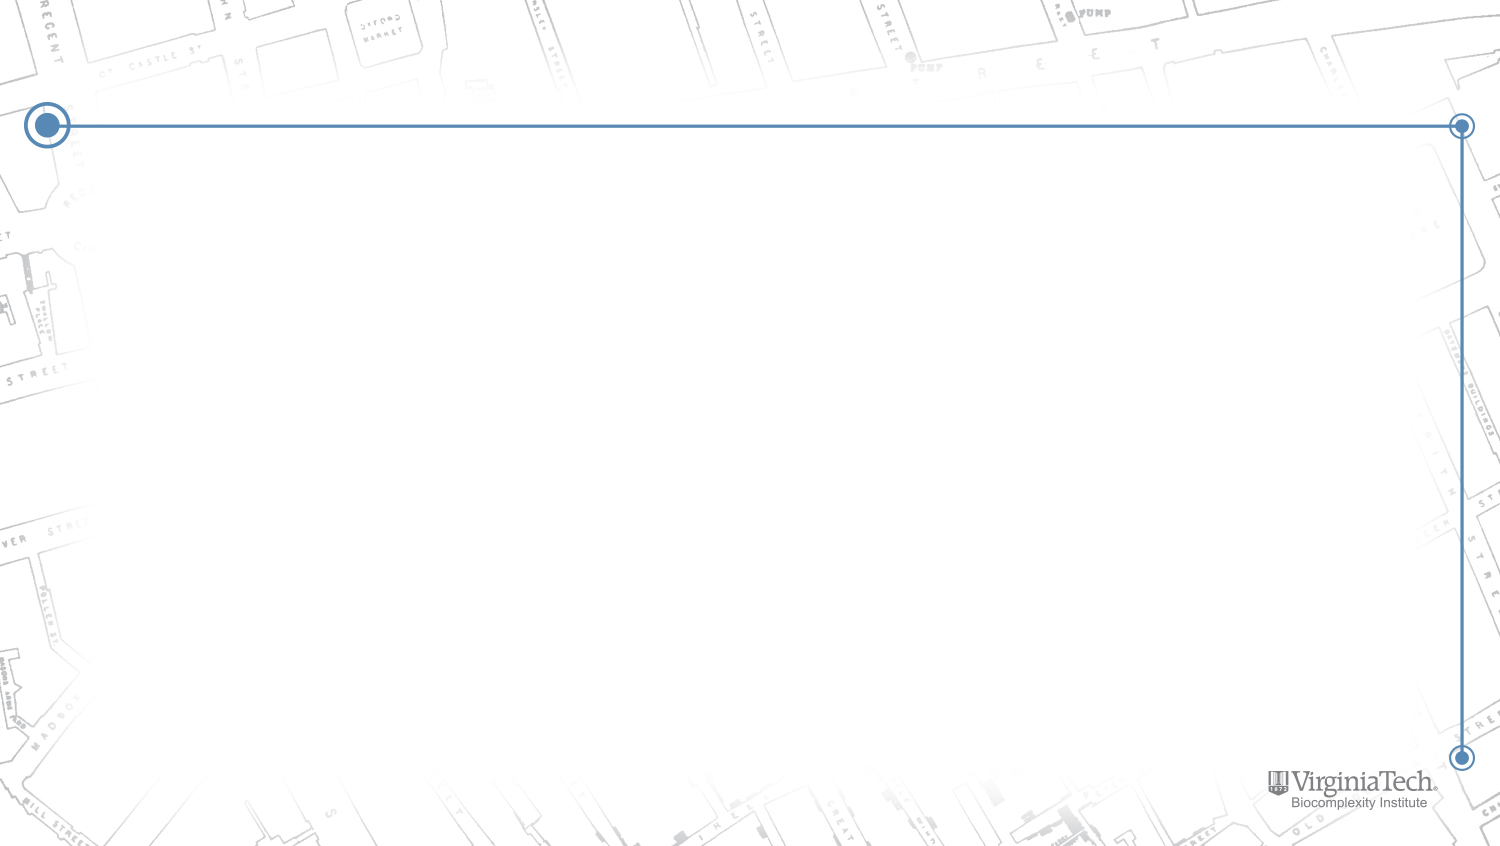
\includegraphics[height=\paperheight,width=\paperwidth]{Template/slides/Basic2Logo.jpg}}
\setbeamertemplate{frametitle}
{\begin{flushright}\vspace{.23in}{\insertframetitle\hspace{.2in}}\end{flushright}}
\setbeamertemplate{footline}{}
}
\makeatother

% Basic3Logo

\makeatletter
\define@key{beamerframe}{Basic3Logo}[true]{%
\usebackgroundtemplate{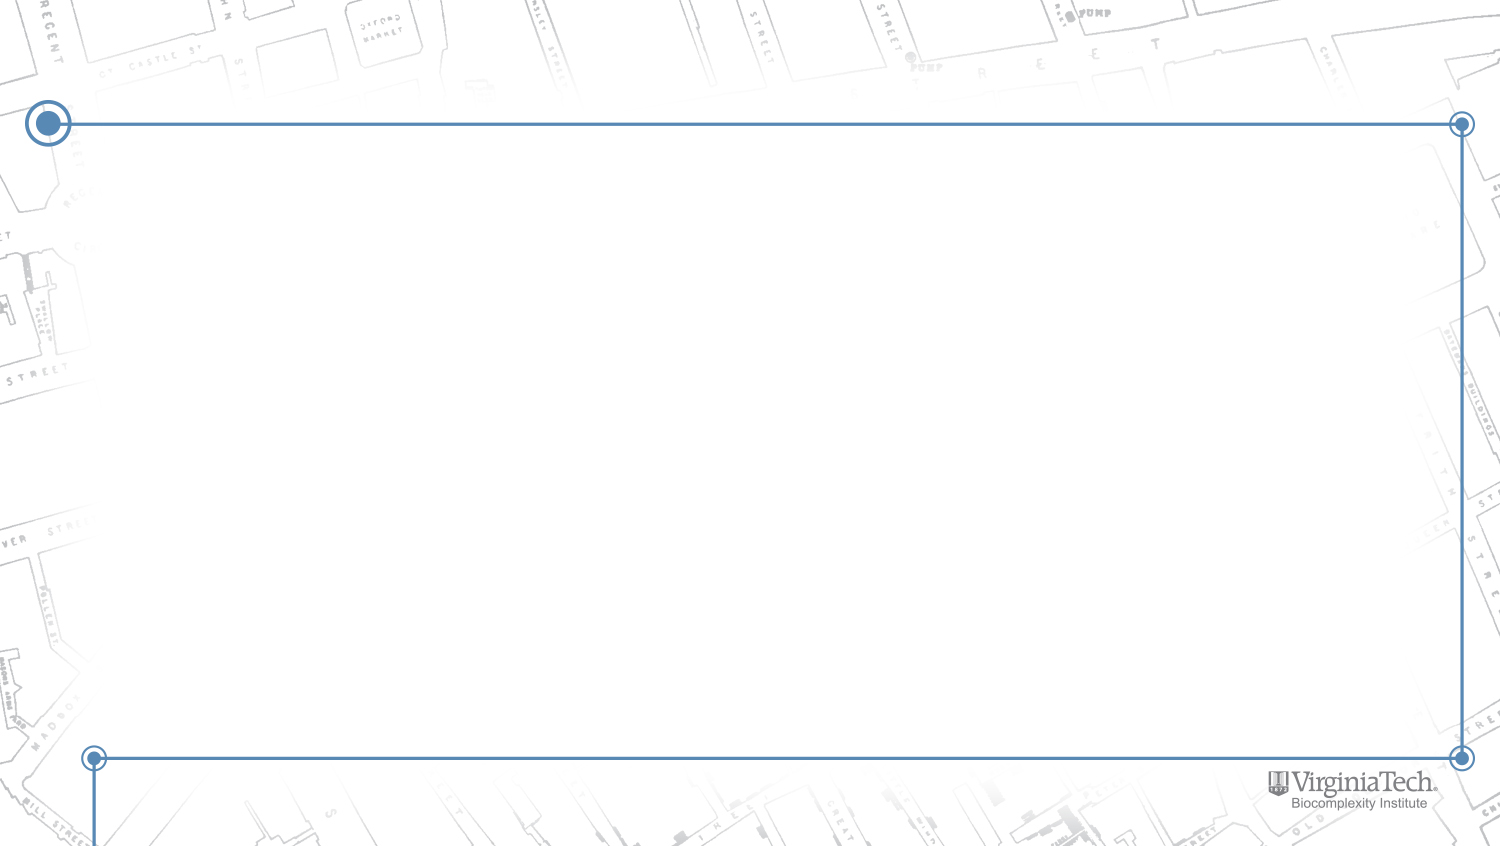
\includegraphics[height=\paperheight,width=\paperwidth]{Template/slides/Basic3Logo.jpg}}
\setbeamertemplate{frametitle}
{\begin{flushright}\vspace{.23in}{\insertframetitle\hspace{.2in}}\end{flushright}}
\setbeamertemplate{footline}{}
}
\makeatother

% Section

\makeatletter
\define@key{beamerframe}{Section}[true]{%
%\setbeamertemplate{frametitle}[default][right]
%\addtobeamertemplate{frametitle}{\vskip1.4in\hspace*{-.7in}}{}
\usebackgroundtemplate{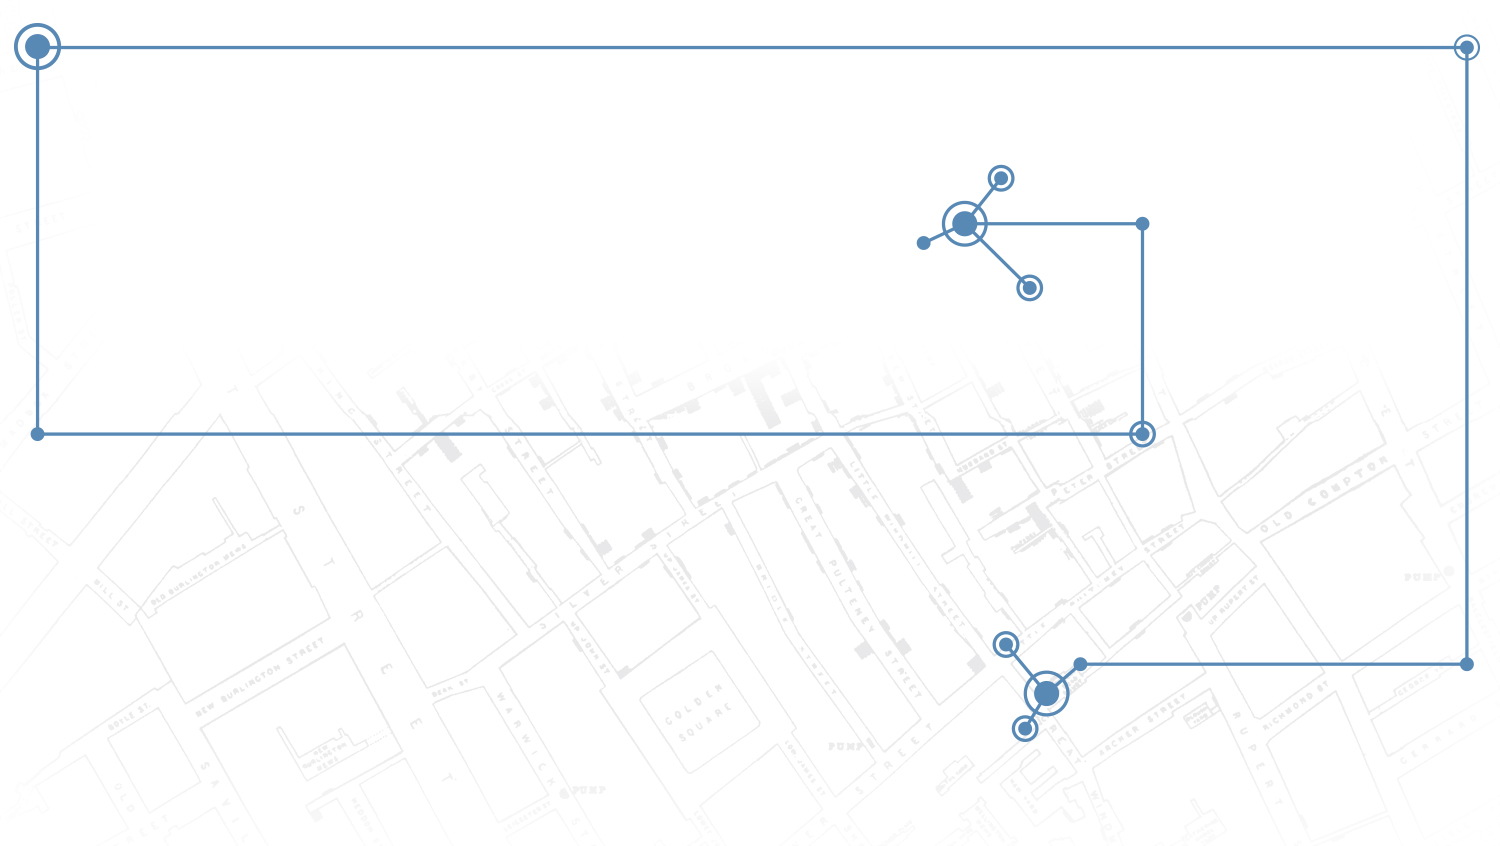
\includegraphics[height=\paperheight,width=\paperwidth]{Template/slides/Section.jpg}}
\hspace*{-1.8in}
\setbeamertemplate{frametitle}
{\begin{flushright}\vskip1.5in{\insertframetitle}\end{flushright}}
\setbeamertemplate{footline}{}
}
\makeatother

\mode
<all>


% This file includes instructions on how to use the template
% e.g., how to call up specific frame formats

% The necessary packages are already loaded within the .sty document. 
% You must add specific ones if needed depending on your needs.

%%%%%%%%%%%%%%%%%%%%%%%%%%%%%%
%%%%%%%%%%%%%%%%%%%%%%%%%%%%%%

\documentclass[compress]{beamer}
\ProvidesPackageRCS $Header: SDAL_Beamer.sty ,v 1 05/13/2016 $

\mode<presentation>

% Set presentation size

\usepackage[orientation=landscape,size=custom,width=16,height=9,scale=0.5,debug]{beamerposter} 
\setbeamersize{text margin left=.25in,text margin right=.25in}

% Set Fonts

%\usepackage[T1]{fontenc}
%\usepackage[default]{raleway}
 
 \usefonttheme{serif}
 
 \setbeamerfont{frametitle}{series=\bfseries} 
\setbeamerfont{title}{series=\bfseries} 
\setbeamerfont{author}{series=\bfseries} 

%\usepackage[T1]{fontenc}
%\usepackage[nosfdefault]{raleway}

% Set the size of the font

\usepackage{scrextend}
\changefontsizes{14pt}
\setbeamerfont{title}{size=\fontsize{17pt}{17pt}}
\setbeamerfont{author}{size=\fontsize{14pt}{14pt}}
\setbeamerfont{frametitle}{size=\fontsize{17pt}{17pt}}
\setbeamerfont{date}{size=\fontsize{14pt}{14pt}}
\setbeamerfont*{structure}{size*={17pt}{17pt}}
\setbeamerfont*{tiny structure}{size*={6pt}{6pt}}
  
% Table of Contents

\setbeamertemplate{section in toc}[ball]
\setbeamertemplate{subsection in toc}[square]

\setbeamertemplate{subsection in toc}{\hspace{1.2em}{\color{BIlightblue}\rule[0.3ex]{6pt}{6pt}}~\inserttocsubsection\par}

% Set Color

\definecolor{VTmaroon}{RGB}{102,0,0} 
\definecolor{VTorange}{RGB}{255,102,0}
\definecolor{BIdarkblue}{RGB}{18,37,45}
\definecolor{BIaquablue}{RGB}{126,168,173}
\definecolor{BIcoolgrey}{RGB}{153,153,153}
\definecolor{BIlightblue}{RGB}{93,137,180}
\definecolor{BIlightgreen}{RGB}{141,194,136}

 
\setbeamercolor*{title}{fg=black}
\setbeamercolor{author}{fg=black} 
\setbeamercolor{frametitle}{fg=black} 
\setbeamercolor{section in toc}{fg=black}
\setbeamercolor{subsection in toc}{fg=black}
\setbeamercolor{itemize subsubitem}{fg=black}
\setbeamercolor{itemize subitem}{fg=black}
\setbeamercolor{itemize item}{fg=black}
\setbeamercolor{section number projected}{bg=BIlightblue,fg=white}

% Lists

\makeatletter
\renewcommand{\itemize}[1][]{%
  \beamer@ifempty{#1}{}{\def\beamer@defaultospec{#1}}%
  \ifnum \@itemdepth >2\relax\@toodeep\else
    \advance\@itemdepth\@ne
    \beamer@computepref\@itemdepth% sets \beameritemnestingprefix
    \usebeamerfont{itemize/enumerate \beameritemnestingprefix body}%
    \usebeamercolor[fg]{itemize/enumerate \beameritemnestingprefix body}%
    \usebeamertemplate{itemize/enumerate \beameritemnestingprefix body begin}%
    \list
      {\usebeamertemplate{itemize \beameritemnestingprefix item}}
      {%
        \setlength\topsep{0pt}%NEW
        \setlength\partopsep{0pt}%NEW
        \setlength\itemsep{0pt}%NEW
        \def\makelabel##1{%
          {%
            \hss\llap{{%
                \usebeamerfont*{itemize \beameritemnestingprefix item}%
                \usebeamercolor[fg]{itemize \beameritemnestingprefix item}##1}}%
          }%
        }%
      }
  \fi%
  \beamer@cramped%
  \raggedright%
  \beamer@firstlineitemizeunskip%
}
\makeatother

\setlength\topsep{-10pt}
\setlength\partopsep{-10pt}


\setbeamertemplate{itemize items}[circle]
\setbeamertemplate{itemize subitem}{---}
\setbeamertemplate{itemize subsubitem}[circle]

% TOC

\makeatletter
\patchcmd{\beamer@sectionintoc}
  {\vfill}
  {\vskip\itemsep}
  {}
  {}
\makeatother  

% Remove navigation symbols

\setbeamertemplate{navigation symbols}{}

% Format Title Page

\defbeamertemplate*{title page}{customized}[1][]
{
\centering
\vspace{.9in}\hspace*{-3.8in}
\begin{overlayarea}{4.1in}{1cm}
\centering{
\usebeamerfont{title}\inserttitle\par}
\usebeamerfont{subtitle}\usebeamercolor[fg]{subtitle}\insertsubtitle\par
\end{overlayarea}\\
\vspace{.2in}\hspace*{-1in}
\begin{overlayarea}{4in}{1cm}
\centering{
\usebeamerfont{date}\insertdate\par \vspace{.1in}
\usebeamerfont{author}\insertauthor\par
\usebeamerfont{institute}\insertinstitute\par}
\end{overlayarea}
}

%%% Formatting Different Frame Styles

% Title

\makeatletter
\define@key{beamerframe}{Title}[true]{%
\usebackgroundtemplate{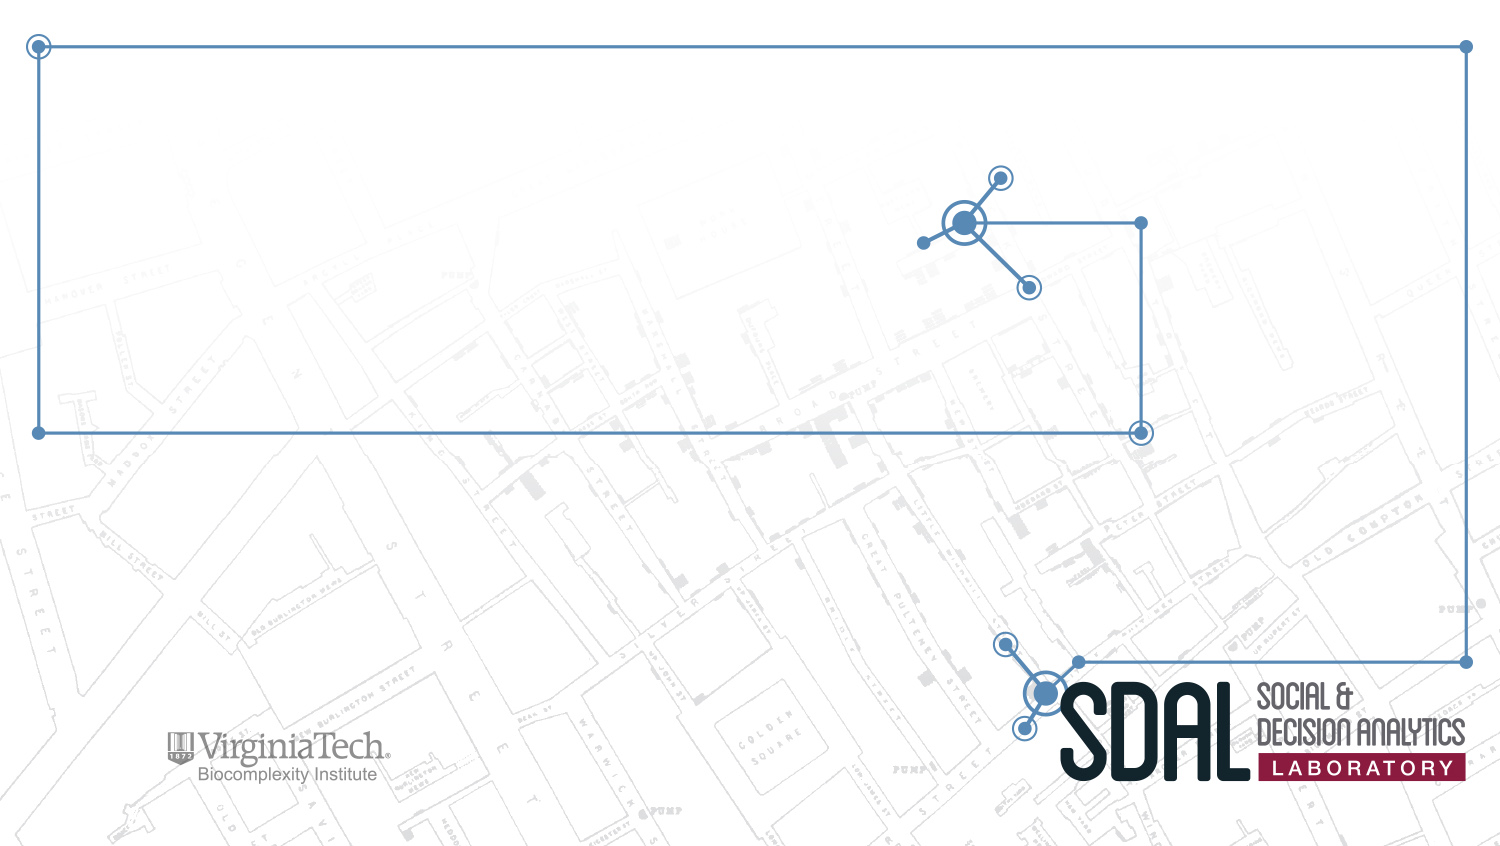
\includegraphics[height=\paperheight,width=\paperwidth]{Template/slides/Title.jpg}
\setbeamertemplate{frametitle}[default][right]
\addtobeamertemplate{frametitle}{\vskip.1in\hspace*{.5in}}{}}
\setbeamertemplate{footline}{}
}
\makeatother

% Outline

\makeatletter
\define@key{beamerframe}{ToC}[true]{%
\usebackgroundtemplate{
\includegraphics[height=\paperheight,width=\paperwidth]{Template/slides/Blank.jpg}}
\setbeamertemplate{frametitle}[default][right]
\addtobeamertemplate{frametitle}{\vskip.1in\hspace*{.5in}}{}
\setbeamertemplate{footline}{}
}
\makeatother

% Blank

\makeatletter
\define@key{beamerframe}{Blank}[true]{%
\usebackgroundtemplate{
\includegraphics[height=\paperheight,width=\paperwidth]{Template/slides/Blank.jpg}}
\setbeamertemplate{frametitle}
{\begin{flushright}\vspace{.23in}{\insertframetitle\hspace{.2in}}\end{flushright}}
\setbeamertemplate{footline}{%
\leavevmode%
  \hbox{%
    \begin{beamercolorbox}[wd=\paperwidth,ht=2.5ex,dp=1.125ex]{palette quaternary}%
    \vspace{.08in}\insertnavigation{\paperwidth}{}{\hskip0pt plus1filll}
    \end{beamercolorbox}%
  }
}
}
\makeatother

% BlankLogo

\makeatletter
\define@key{beamerframe}{BlankLogo}[true]{%
\usebackgroundtemplate{
\includegraphics[height=\paperheight,width=\paperwidth]{Template/slides/BlankLogo.jpg}}
\setbeamertemplate{frametitle}
{\begin{flushright}\vspace{.23in}{\insertframetitle\hspace{.2in}}\end{flushright}}
\setbeamertemplate{footline}{}
}
\makeatother

% Basic1

\makeatletter
\define@key{beamerframe}{Basic1}[true]{%
\usebackgroundtemplate{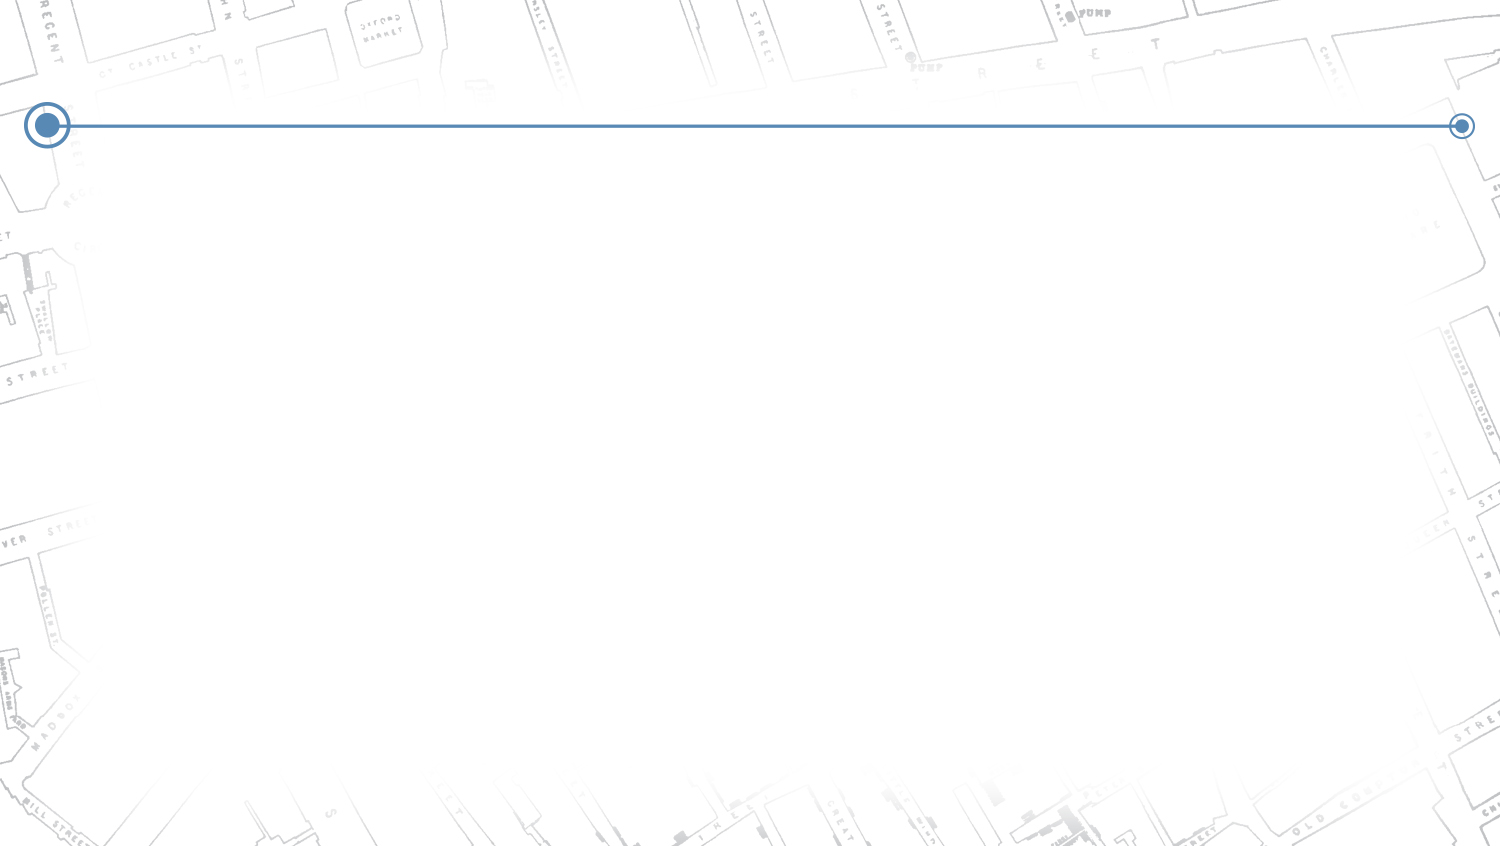
\includegraphics[height=\paperheight,width=\paperwidth]{Template/slides/Basic1.jpg}}
\setbeamertemplate{frametitle}
{\begin{flushright}\vspace{.23in}{\insertframetitle\hspace{.2in}}\end{flushright}}
\setbeamertemplate{footline}{%
\leavevmode%
  \hbox{%
    \begin{beamercolorbox}[wd=\paperwidth,ht=2.5ex,dp=1.125ex]{palette quaternary}%
    \vspace{.08in}\insertnavigation{\paperwidth}{}{\hskip0pt plus1filll}
    \end{beamercolorbox}%
  }
}
}
\makeatother

% Basic2

\makeatletter
\define@key{beamerframe}{Basic2}[true]{%
\usebackgroundtemplate{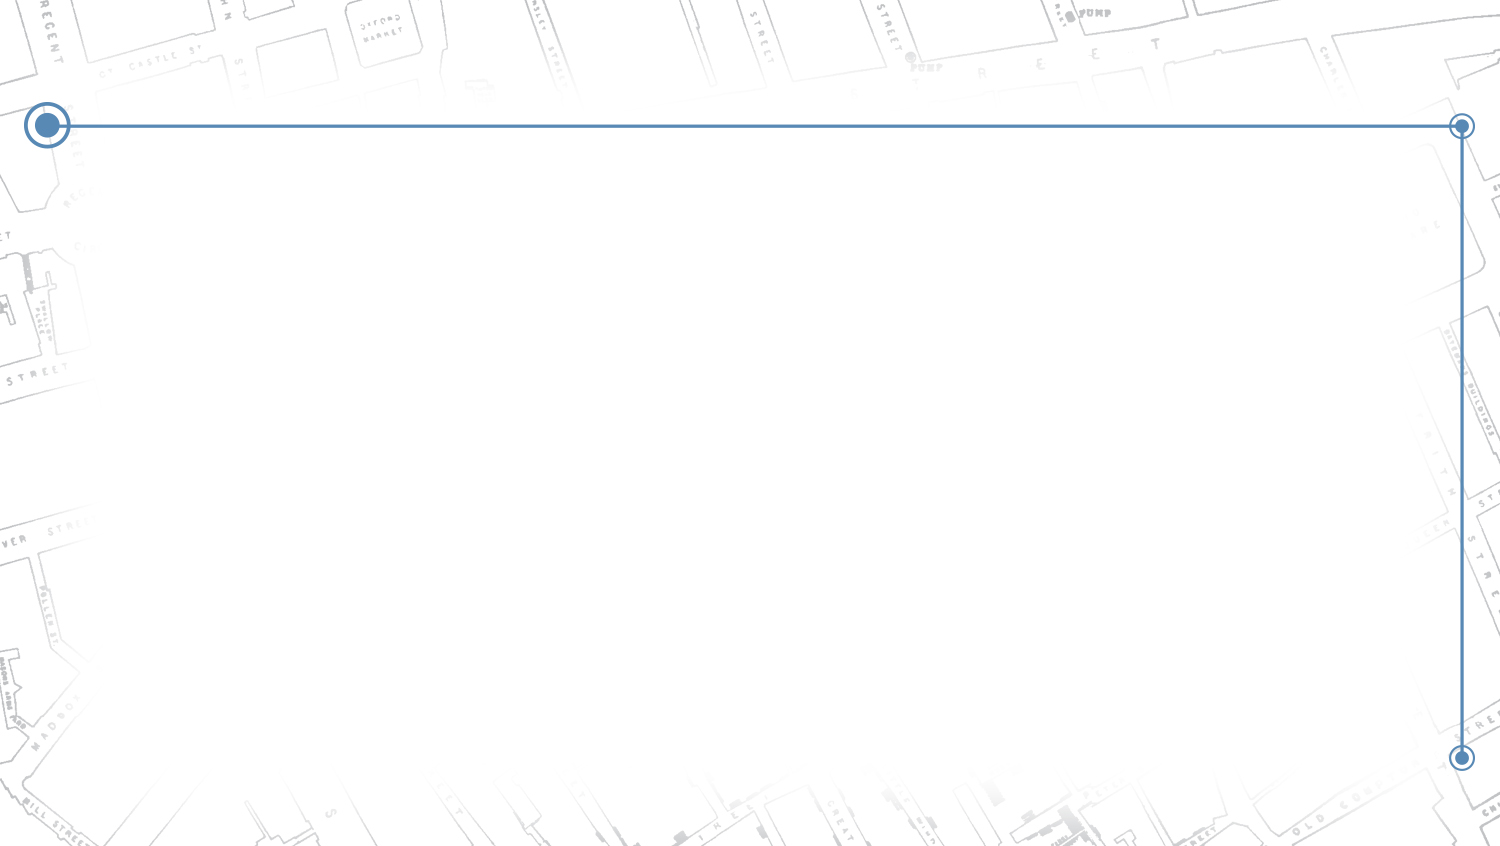
\includegraphics[height=\paperheight,width=\paperwidth]{Template/slides/Basic2.jpg}}
\setbeamertemplate{frametitle}
{\begin{flushright}\vspace{.23in}{\insertframetitle\hspace{.2in}}\end{flushright}}
\setbeamertemplate{footline}{%
\leavevmode%
  \hbox{%
    \begin{beamercolorbox}[wd=\paperwidth,ht=2.5ex,dp=1.125ex]{palette quaternary}%
    \vspace{.08in}\insertnavigation{\paperwidth}{}{\hskip0pt plus1filll}
    \end{beamercolorbox}%
  }
}
}
\makeatother

% Basic3

\makeatletter
\define@key{beamerframe}{Basic3}[true]{%
\usebackgroundtemplate{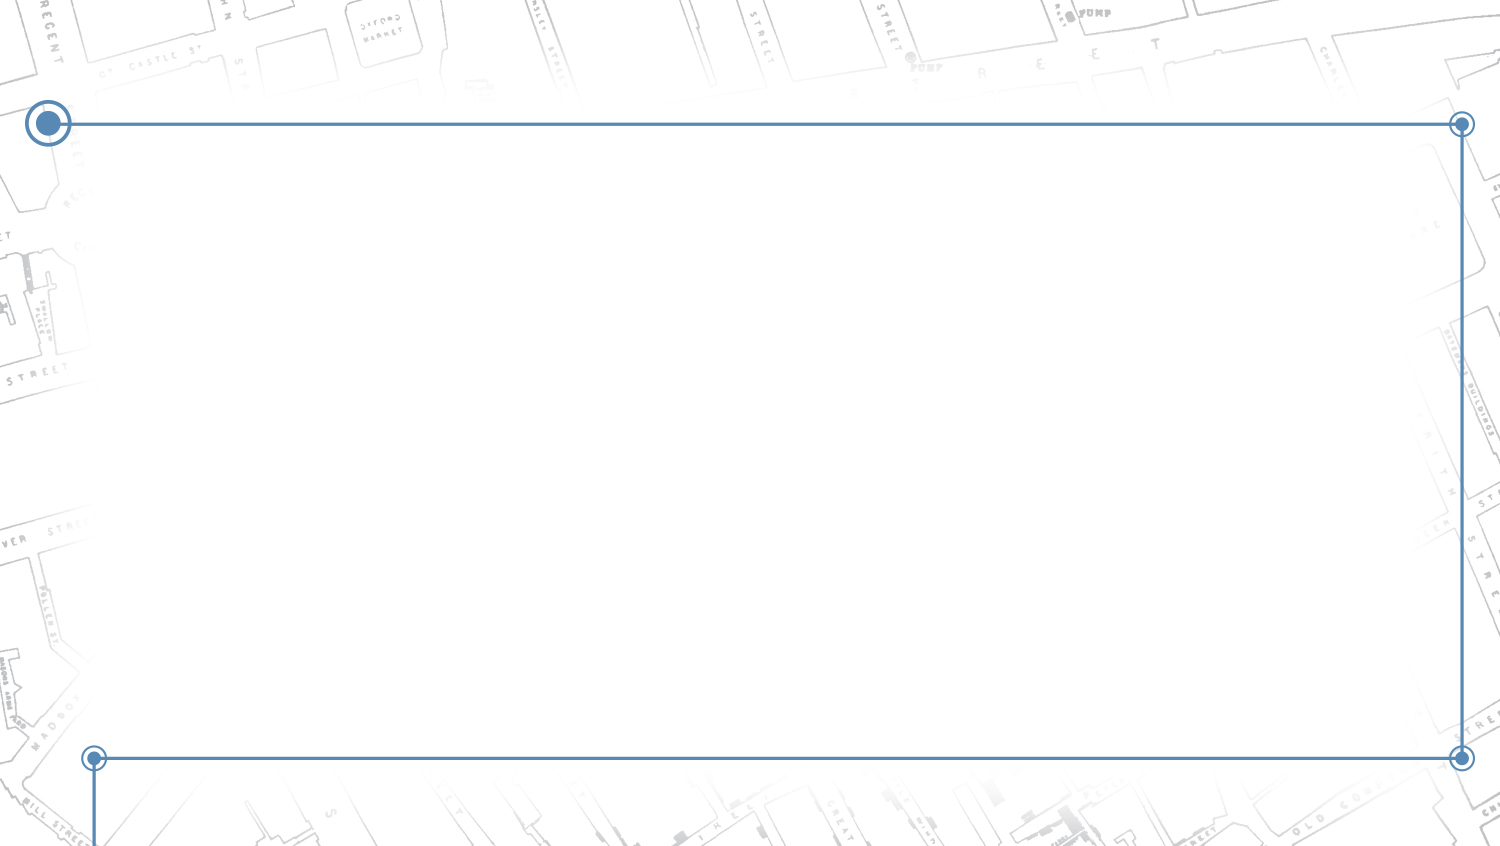
\includegraphics[height=\paperheight,width=\paperwidth]{Template/slides/Basic3.jpg}}
\setbeamertemplate{frametitle}
{\begin{flushright}\vspace{.23in}{\insertframetitle\hspace{.2in}}\end{flushright}}
\setbeamertemplate{footline}{}
}
\makeatother

% Basic1Logo

\makeatletter
\define@key{beamerframe}{Basic1Logo}[true]{%
\usebackgroundtemplate{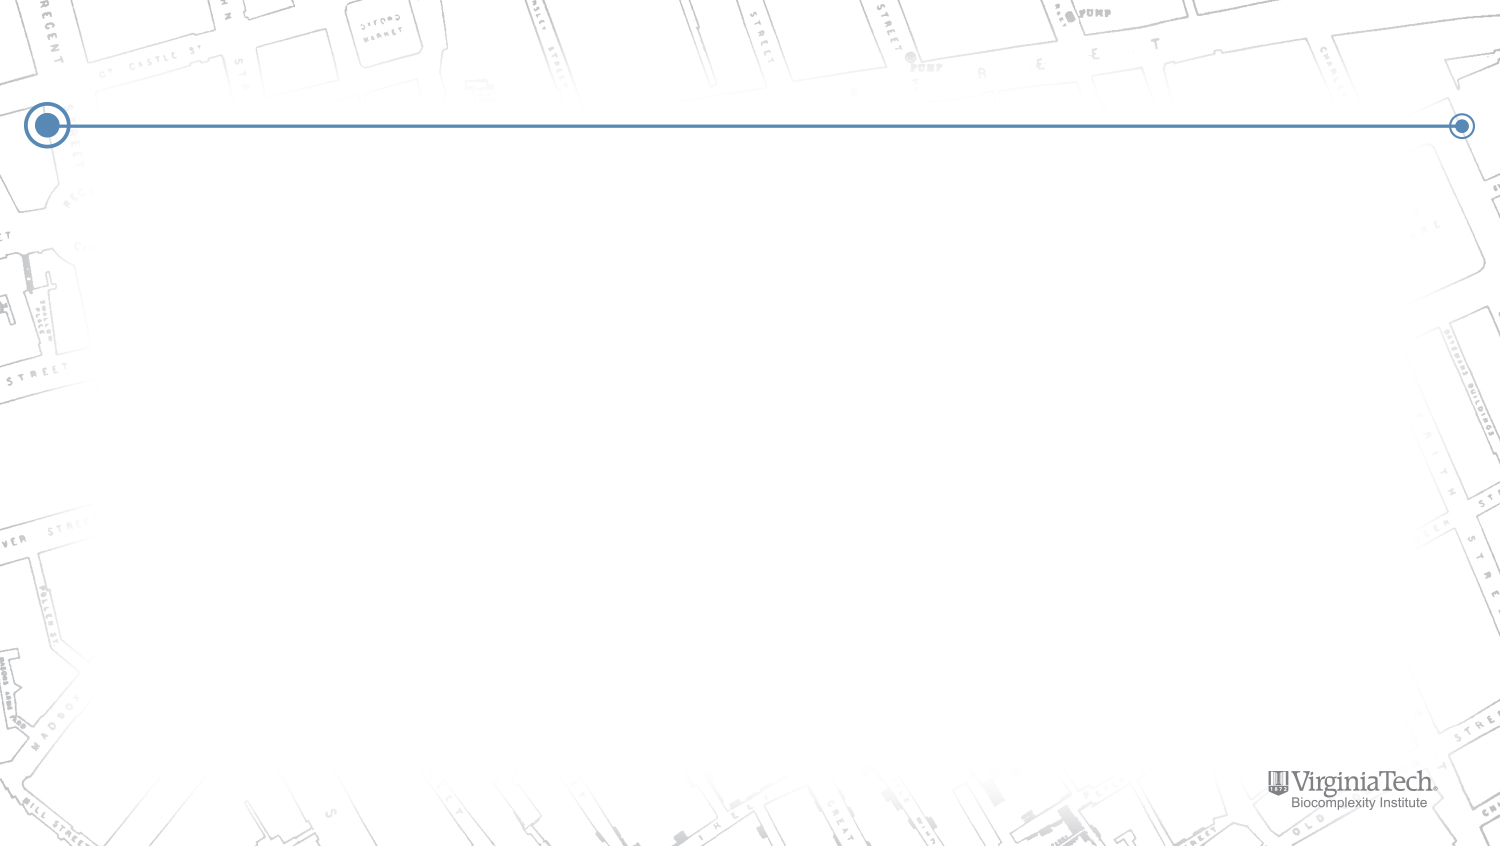
\includegraphics[height=\paperheight,width=\paperwidth]{Template/slides/Basic1Logo.jpg}}
\setbeamertemplate{frametitle}
{\begin{flushright}\vspace{.23in}{\insertframetitle\hspace{.2in}}\end{flushright}}
\setbeamertemplate{footline}{}
}
\makeatother

% Basic2Logo

\makeatletter
\define@key{beamerframe}{Basic2Logo}[true]{%
\usebackgroundtemplate{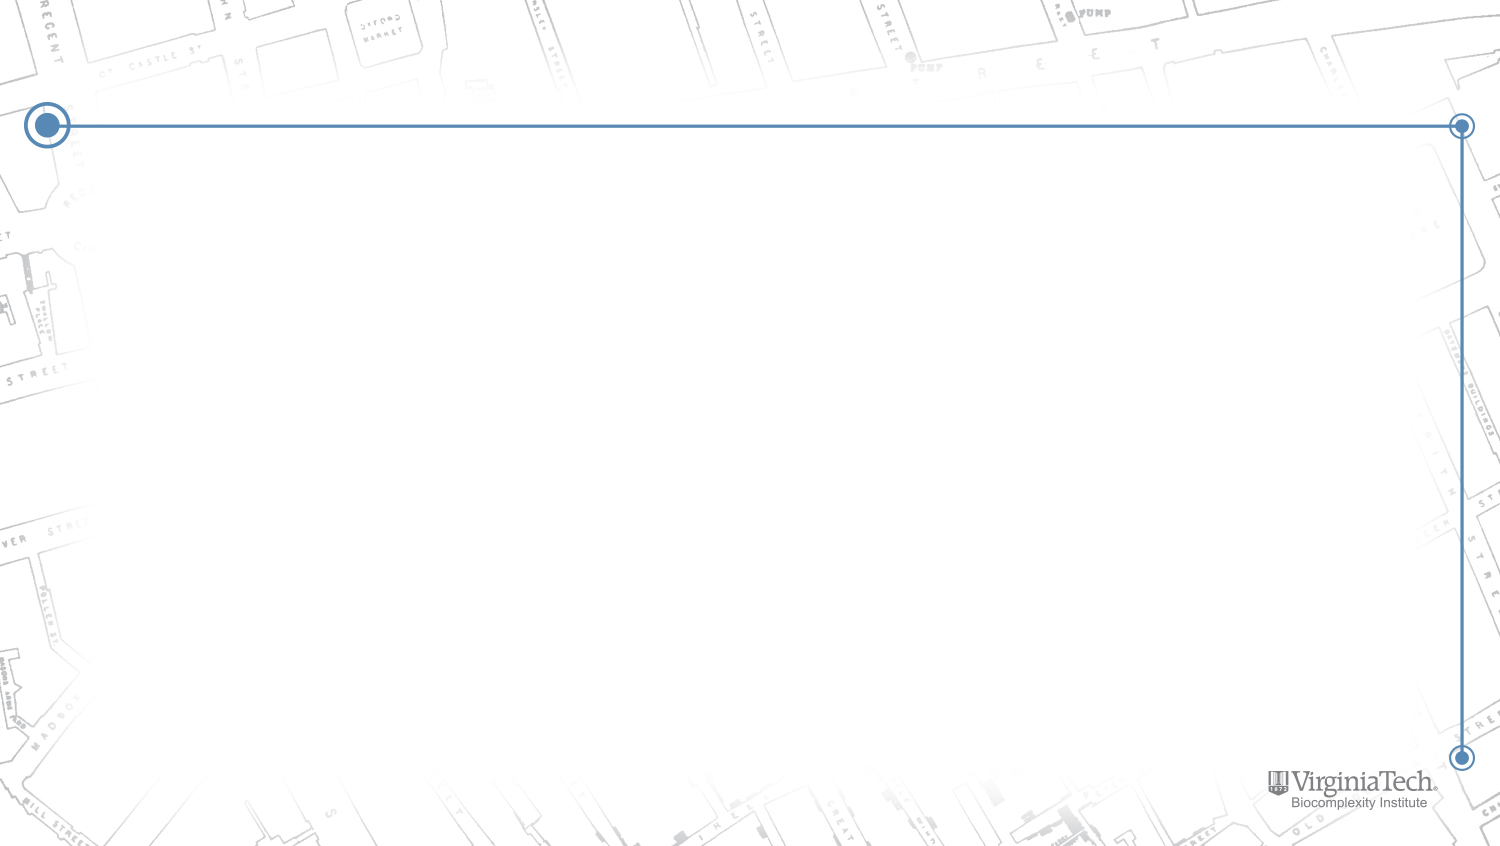
\includegraphics[height=\paperheight,width=\paperwidth]{Template/slides/Basic2Logo.jpg}}
\setbeamertemplate{frametitle}
{\begin{flushright}\vspace{.23in}{\insertframetitle\hspace{.2in}}\end{flushright}}
\setbeamertemplate{footline}{}
}
\makeatother

% Basic3Logo

\makeatletter
\define@key{beamerframe}{Basic3Logo}[true]{%
\usebackgroundtemplate{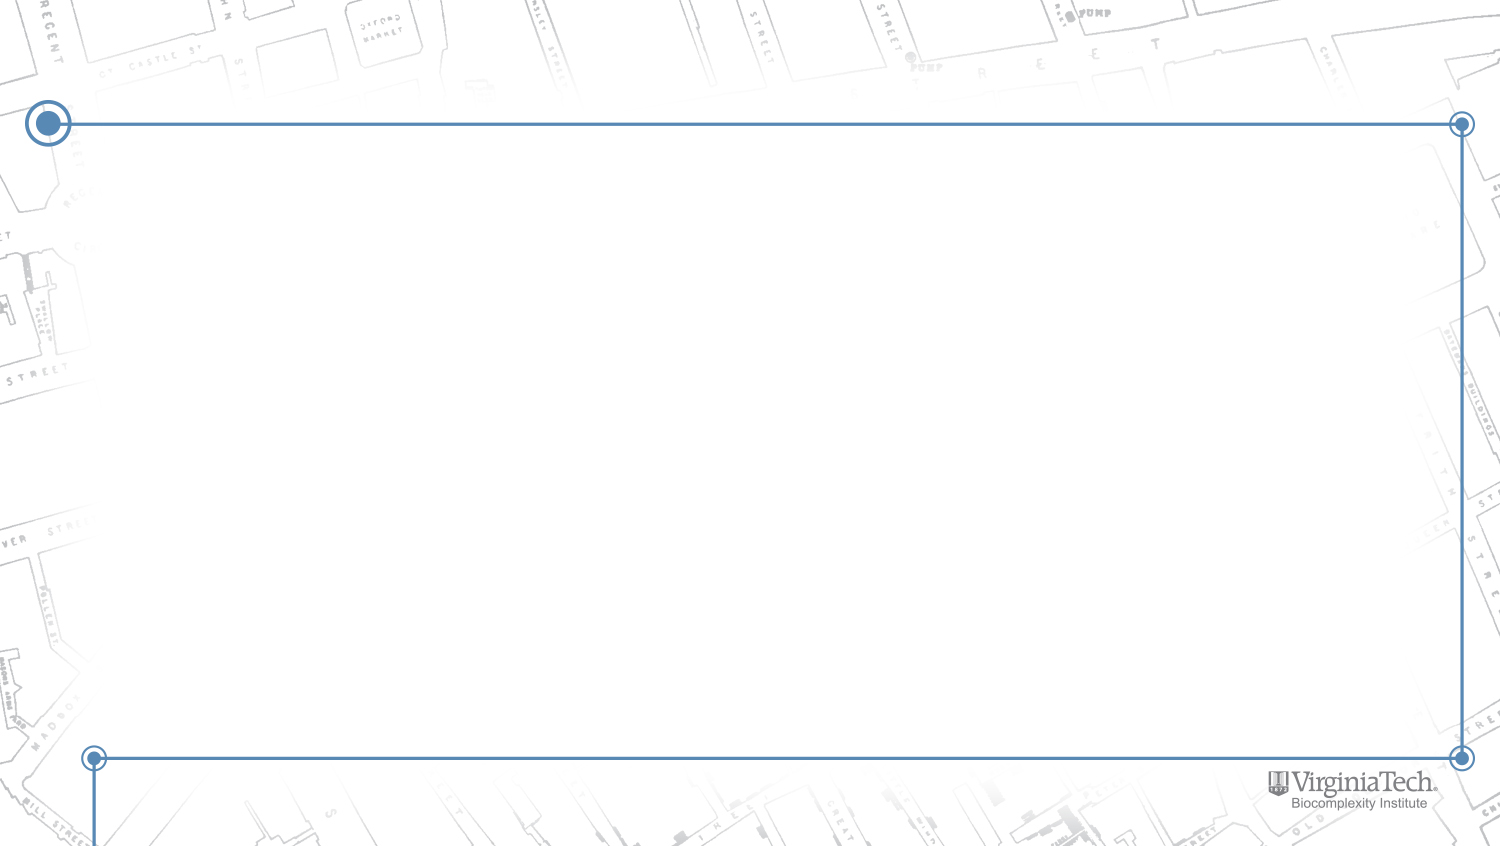
\includegraphics[height=\paperheight,width=\paperwidth]{Template/slides/Basic3Logo.jpg}}
\setbeamertemplate{frametitle}
{\begin{flushright}\vspace{.23in}{\insertframetitle\hspace{.2in}}\end{flushright}}
\setbeamertemplate{footline}{}
}
\makeatother

% Section

\makeatletter
\define@key{beamerframe}{Section}[true]{%
%\setbeamertemplate{frametitle}[default][right]
%\addtobeamertemplate{frametitle}{\vskip1.4in\hspace*{-.7in}}{}
\usebackgroundtemplate{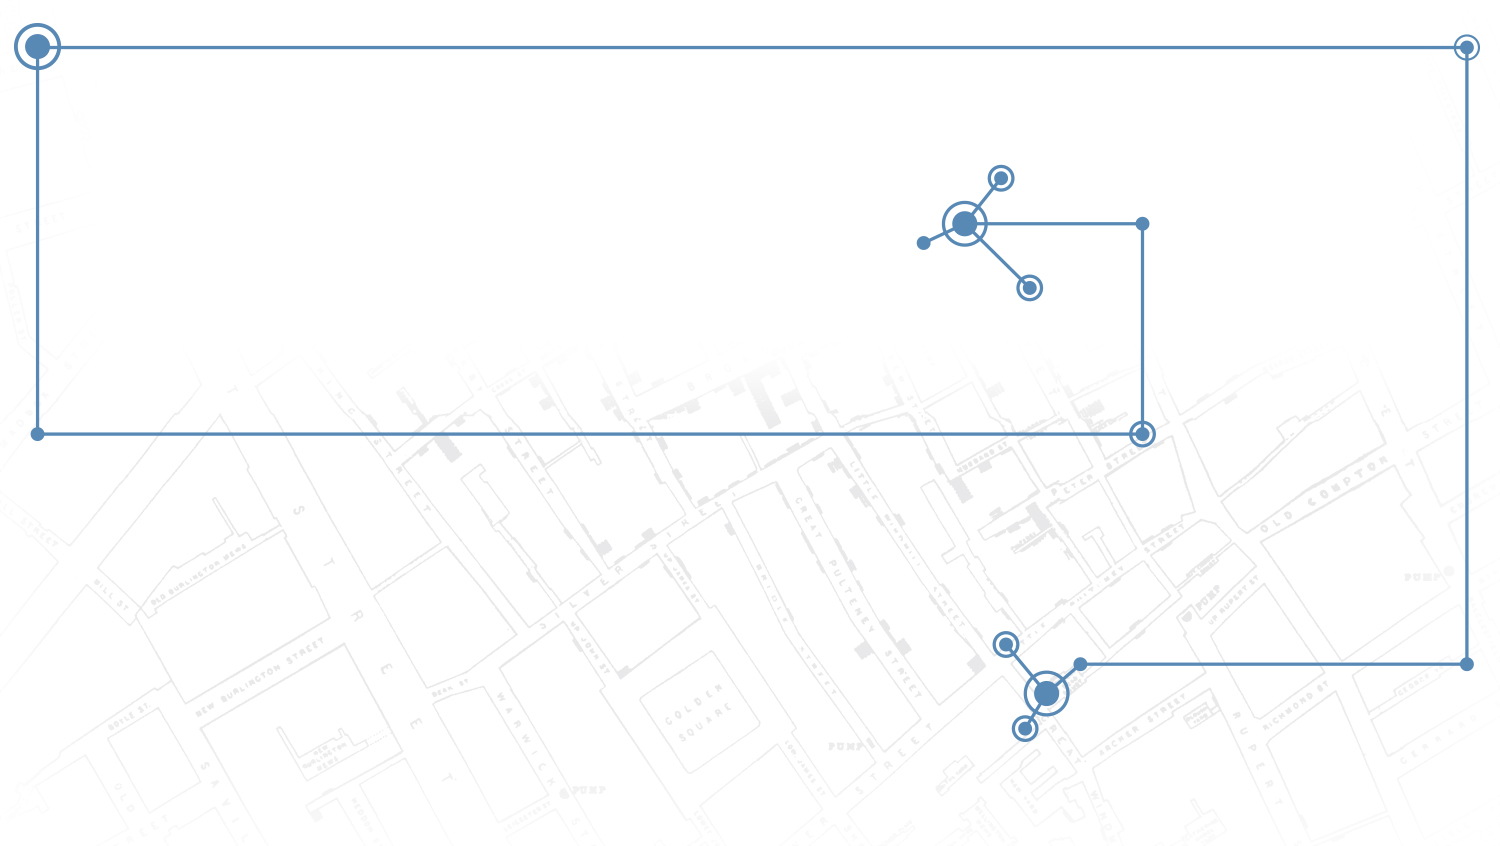
\includegraphics[height=\paperheight,width=\paperwidth]{Template/slides/Section.jpg}}
\hspace*{-1.8in}
\setbeamertemplate{frametitle}
{\begin{flushright}\vskip1.5in{\insertframetitle}\end{flushright}}
\setbeamertemplate{footline}{}
}
\makeatother

\mode
<all>


\usepackage[english]{babel}

\usepackage{csquotes}

\usepackage[pscoord]{eso-pic}% The zero point of the coordinate systemis the lower left corner of the page (the default).

\newcommand{\placetextbox}[3]{% \placetextbox{<horizontal pos>}{<vertical pos>}{<stuff>}
	\setbox0=\hbox{#3}% Put <stuff> in a box
	\AddToShipoutPictureFG*{% Add <stuff> to current page foreground
		\put(\LenToUnit{#1\paperwidth},\LenToUnit{#2\paperheight}){\vtop{{\null}\makebox[0pt][c]{#3}}}%
	}%
}%

\usepackage{caption}
\captionsetup[figure]{labelformat=empty}% redefines the caption setup of the figures environment in the beamer class.


% Template Colors: VTmaroon, VTorange, BIdarkblue, BIaquablue, BIcoolgrey, BIlightblue, BIlightgreen

\title[SDAL]{\vspace{-0.85in}Changing People's Minds: Understanding Social Diffusion Dynamics Using Networked Cognitive Systems}
\author{Daniel Chen, MPH\\ \tiny{Computational. Network. Epidemiology}}
\date[]{September 1, 2016}

% For long titles and/or subtitles, will need to use \vspace[-XXin] to align accordingly

\begin{document}

	\begin{frame}[BlankLogo] \frametitle{}
		\begin{figure}
	\centering
	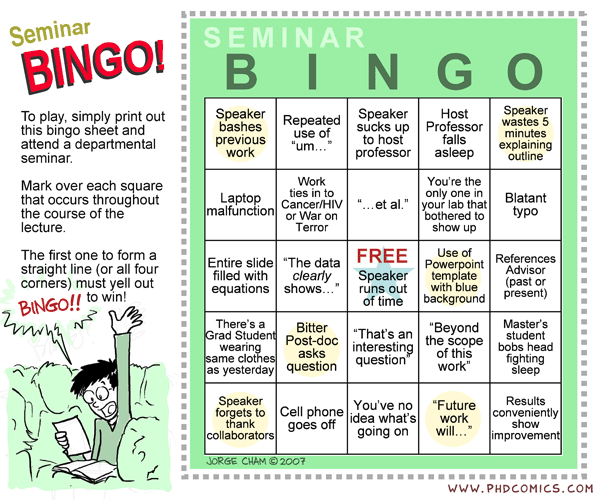
\includegraphics[height=0.9\textheight]{../phd040907s_bingo}
	\label{fig:phd040907sbingo}
	\end{figure}
	
	\end{frame}
	
	\begin{frame}[Title]
		\titlepage
	\end{frame}

% If you do not want an outline, do not include this slide
% Edit toc depth for what level you want included

%	\begin{frame}[ToC] \frametitle{Outline}
%	\setcounter{tocdepth}{2}
%	\hfill
%	\parbox[t]{.95\textwidth}{
%		\begin{minipage}[c][0.75\textheight]{\textwidth}
%			\linespread{1}
%			\tableofcontents
%		\end{minipage}
%	}
%	\end{frame}

% Note on progress tracker:
% If you do not want the progress tracker in the footer, do not use \section or \subsections
% Progress tracker online works on Blank, Basic 1 and Basic 2 slide types

% Compile twice after adding sections and subsection to get them to appear
% Subsections are represented by the dots in the footer. Do not use sections if you do not want the dots.
% Place subsections right above that slide to have dots highlight appropriately

\section[SDAL]{SDAL}

	\begin{frame}[Section] \frametitle{\vspace{-0.2in}Social \& Decision Analytics\\Laboratory}
	\end{frame}

\subsection[Social and Decision Analytics Laboratory (SDAL)]{Social and Decision Analytics Laboratory (SDAL)}

	\begin{frame}[Basic2] \frametitle{The Social and Decision Analytics Laboratory}
		Founded in 2013
		\vspace{3mm}

		\begin{columns}
			\begin{column}{0.5\textwidth}
				\begin{figure}
					\centering
					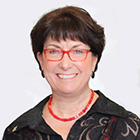
\includegraphics[width=2cm]{../figures/keller-sallie-140-w}
					\caption{Sallie Keller\\Director\\Professor}
					\label{fig:keller-sallie-140-w}
				\end{figure}
			\end{column}
			\begin{column}{0.5\textwidth}  %%<--- here
				\begin{figure}
					\centering
					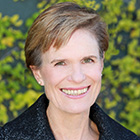
\includegraphics[width=2cm]{../figures/shipp-stephanie-140-w}
					\begin{center}
						\caption{Stephanie Shipp\\Deputy Director\\Research Professor}
					\end{center}
					\label{fig:shipp-stephanie-140-w}
				\end{figure}
			\end{column}
		\end{columns}

		\begin{displayquote}
		statisticians and social and behavioral scientists to embrace today’s data revolution, developing evidence-based research and quantitative methods to inform policy decision-making.
		\end{displayquote}
	\end{frame}

	\begin{frame}[Basic2] \frametitle{The Social and Decision Analytics Laboratory}
		\begin{figure}
			\centering
			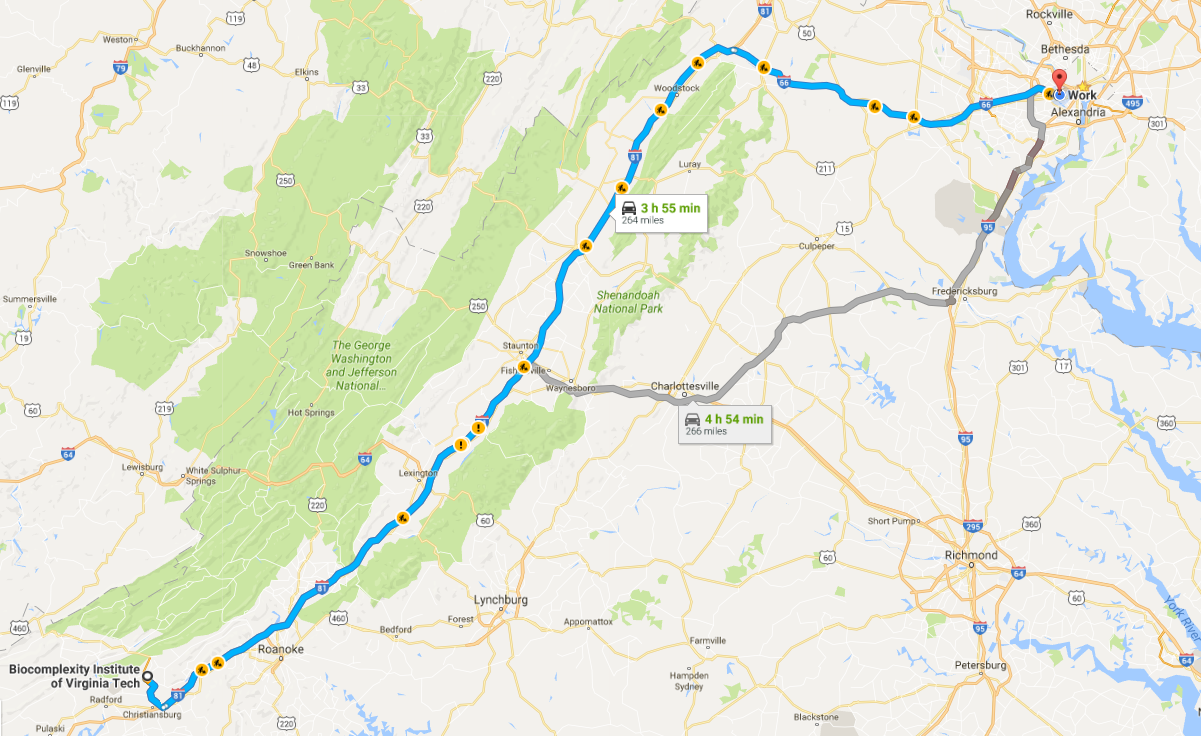
\includegraphics[height=0.75\textheight]{../figures/sdal_google_maps}
			\label{fig:sdalgooglemaps}
		\end{figure}
	\end{frame}

	\begin{frame}[Blank] \frametitle{People}
		\small
		\begin{columns}
			\begin{column}{0.3\textwidth}
				\textbf{Research Faculty}
				\begin{enumerate}
					\item David Higdon (Statistics)
					\item Viki Lancaster (Statistics)
					\item Mark Orr (Psychology)
					\item Aaron Schroeder (Data Science)
					\item Gizem Korkmaz (Economics)
				\end{enumerate}
			\end{column}
		
			\begin{column}{0.3\textwidth}
				\textbf{Post Doctoral Associates}
				\begin{enumerate}
					\item Kathryn Ziemer (Psychology)
					\item Bianica Pires (Social Science)
					\item Emily Molfino (Political Science)
					\item Joshua Goldstein (Statistics)
				\end{enumerate}
			
				\textbf{Visiting Scholars \& Collaborators:} 7
			\end{column}

			\begin{column}{0.3\textwidth}
				\textbf{Students}
				\begin{enumerate}
					\item Daniel Chen (GRA: GBCB)
					\item Adrienne Rogers (VT: Statistics)
					\item Emily Stark (Mathematics)
				\end{enumerate}
				
				\textbf{Administrative Staff}
				\begin{enumerate}
					\item Kimberly Lyman
					\item Tracie Hase
				\end{enumerate}
			\end{column}
		\end{columns}
	\end{frame}

\subsection[Projects]{Projects}

	\begin{frame}[Basic2] \frametitle{Projects}
		\begin{enumerate}
			\item Assessing New Data Sources for the Federal Census
			\item Simulating Urban Air Pollution Exposure
			\item Collaborating to Build a Culture of Health
			\item Leveraging Data to Enhance Emergency Response
			\item Practicing Data Science for the Public Good
			\item Modeling the Spread of Beliefs Through Social Media
		\end{enumerate}
		
	\end{frame}

\subsection[Data Science for the Public Good]{Data Science for the Public Good}

	\begin{frame}[Basic2] \frametitle{Data Science for the Public Good}
		
		\begin{columns}
			\begin{column}{0.5\textwidth}
				\begin{itemize}
					\item First summer for the The Data Science for the Public Good program (DSPG)
					\item Research Experience for Undergraduates (REU) funded by NSF
					\item Bash, SSH, \LaTeX, R, SQL, GIS, Literate Programming, Web Scraping, Git
				\end{itemize}
			\end{column}
			\begin{column}{0.5\textwidth}
				\begin{figure}
					\centering
					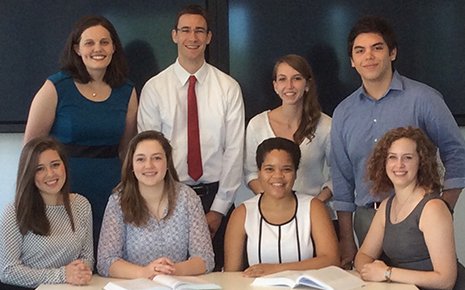
\includegraphics[width=0.9\linewidth]{../figures/data-science-for-public-good-student-photo-overview}
					\caption{My Students! :D}
					\label{fig:data-science-for-public-good-student-photo-overview}
				\end{figure}
			\end{column}
		\end{columns}
	\end{frame}

\subsection[Come Visit]{Come Visit}

	\begin{frame}[Blank] \frametitle{Come Visit!}
		\begin{columns}
			\begin{column}{0.35\textwidth}
				\begin{figure}
					\centering
					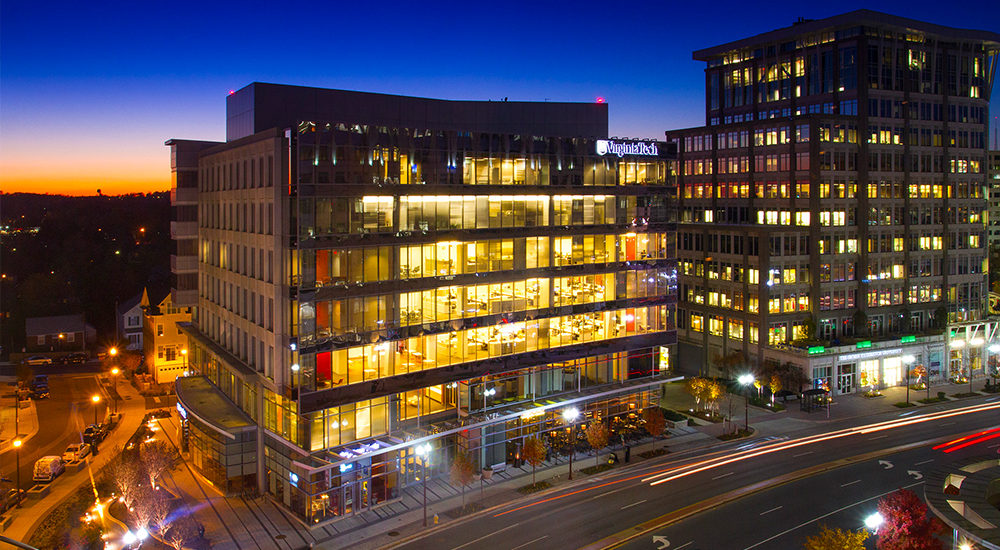
\includegraphics[width=1\linewidth]{../figures/metro-lab-big-data-sdal-header}
					\caption{}
					\label{fig:metro-lab-big-data-sdal-header}
				\end{figure}
				
				\begin{figure}
					\centering
					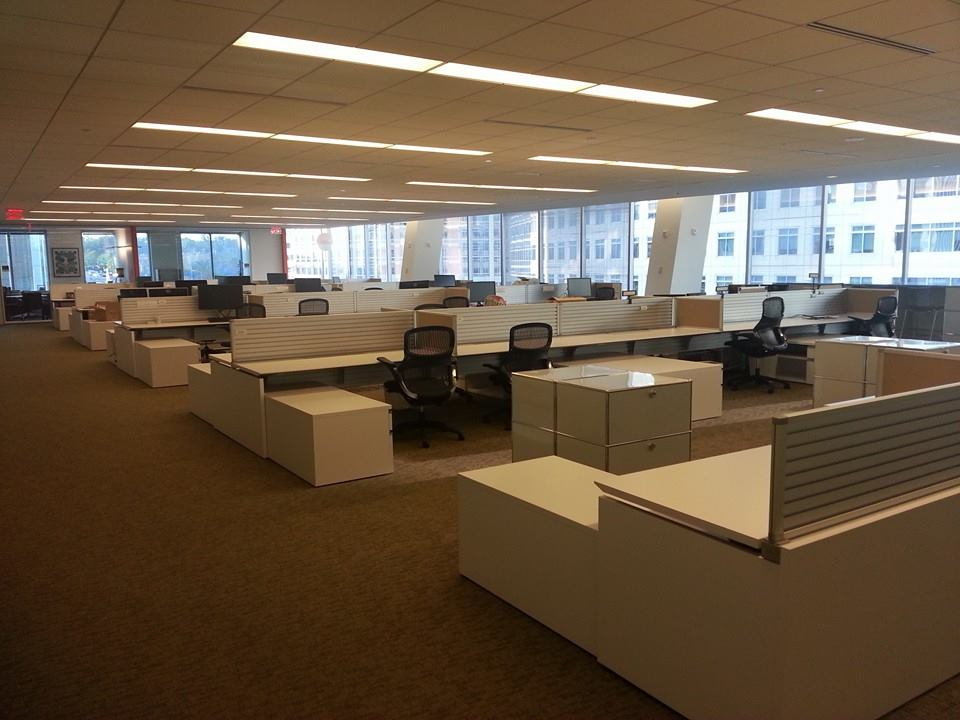
\includegraphics[width=1\linewidth]{../figures/sdal_pit}
					\caption{}
					\label{fig:sdalpit}
				\end{figure}
			\end{column}
						
			\begin{column}{0.65\textwidth}
				\begin{figure}
					\centering
					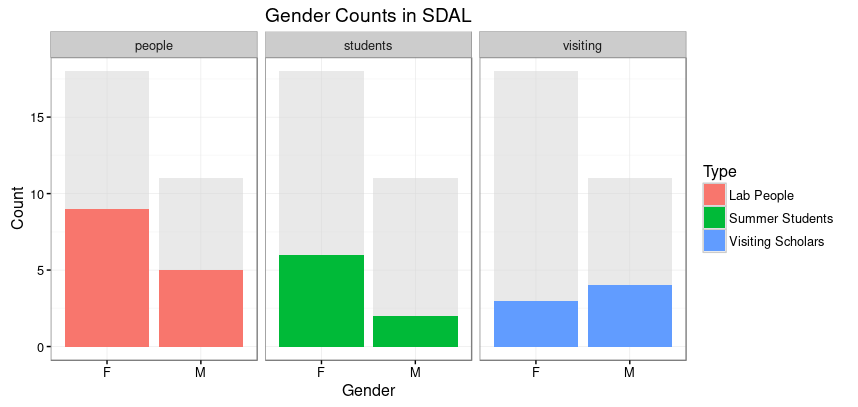
\includegraphics[width=1.0\linewidth]{../figures/sdal_gender_breakdown}
					\caption{}
					\label{fig:sdalgenderbreakdown}
					\end{figure}
			\end{column}
		\end{columns}
	\end{frame}

\section[Introduction]{Introduction}

	\begin{frame}[Section] \frametitle{\vspace{-0.2in}Modeling the Spread of Beliefs\\Through Social Media}
	\end{frame}
	
\subsection[Overview]{Overview}

\begin{frame}[Basic2] \frametitle{Initial Conception}
	\begin{itemize}
		\item Mark Orr, Ph.D.
		\item Columbia University Mailman School of Public Health
		\begin{itemize}
			\item Department of Epidemiology
			\begin{itemize}
				\item Sandro Galea, MD, MPH, DrPH
			\end{itemize}
			\item Columbia University Systems Science Program (CUSSP)
			\begin{itemize}
				\item Mailman School of Public Health (MSPH)
				\item School of Engineering and Applied Sciences (SEAS)
				\item Complex System Approaches in Population Health (CSAPH)
			\end{itemize}
		\end{itemize}
	\end{itemize}
\end{frame}


\begin{frame}[Basic2] \frametitle{Epidemiology}
	merp: the branch of medicine that deals with the incidence, distribution, and possible control of diseases and other factors relating to health.
\end{frame}

\section{Watts}

\section{Neural Networks}

\section{TRA}

\section{ABMs}

\section{Simulations}

\section{Conclusion}

\section{End}

\subsection{Forthcoming Works}
	\begin{frame}[Basic2] \frametitle{Forthcoming Works}
		\begin{itemize}
			\item M. Orr, K. Zeimer, and D. Chen (Forthcoming, Fall 2016). Systems of Behavior and Human Health. In S. Galea \& A. El-Sayed (Eds.), Systems Science and Population Health. Oxford University Press: Oxford, UK.

			\item M. Orr and D. Chen (Forthcoming, Fall 2016). Computational Models of Health Behavior. In R. Vallacher, A. Nowak, and S. Read (Eds.), Computational Models in Social Psychology. Psychology Press/Routledge: New York.
		\end{itemize}
	\end{frame}



\subsection{Thanks!}

	\begin{frame}[Basic2] \frametitle{Thanks!}
		\begin{itemize}
			\item Dennie
			\item GBCB Folks
		\end{itemize}
	
		\begin{itemize}
			\item Mark Orr, PhD
			\item Jacqueline Merrill PhD, MPH, RN, FAAN, FACMI
		\end{itemize}
	
		\begin{itemize}
			\item Mark Orr, PhD
			\item Jacqueline Merrill PhD, MPH, RN, FAAN, FACMI
		\end{itemize}
	\end{frame}
	
\subsection{References}
	\begin{frame}[Basic2] \frametitle{References}
		\tiny
		https://www.bi.vt.edu/sdal/news/student-fellows-in-national-capital-region-learn-to-apply-data-to-solutions
	\end{frame}

\subsection{Links}
	\begin{frame}[Basic2] \frametitle{Thanks!}
		\tiny

		Slides:
		
		Code:
		\begin{itemize}
			\item https://github.com/chendaniely/multi-agent-neural-network
			\item https://github.com/chendaniely/multidisciplinary-diffusion-model-experiments
			\item https://github.com/chendaniely/mann2
			\item https://github.com/chendaniely/mann2\_simulations
			\item https://github.com/chendaniely/mann2\_analysis
		\end{itemize}

		
\includegraphics[width=7mm]{../figures/font-awesome_4-6-3_twitter_256_0_007dff_none}
		@chendaniely

		
\includegraphics[width=7mm]{../figures/brandico_2014-04-07_github_256_0_2c3e50_none}
		www.github.com/chendaniely
	\end{frame}



\end{document}

% Different format names are listed in title slides
% Insert as * in \begin{frame}[*] 

% For long frame titles , will need to use \vspace[-XXin] to align accordingly
% If progress tracker gets in the way for these, can remove from that page using \begin{frame}[FORMAT_NAME,plain]

% If content runs off the slide, the title will move! Split into two slides if this is the case.

\begin{frame}[Blank] \frametitle{Format: Blank}
	This is a test of the template.\\
	The navigation bar on the bottom is optional.
\end{frame}

\begin{frame}[BlankLogo] \frametitle{Format: BlankLogo}
	{\color{VTorange}{This is VTorange}}\\
	{\color{VTmaroon}{This is VTmaroon}}\\
	{\color{BIdarkblue}{This is BIdarkblue}}\\
	{\color{BIaquablue}{This is BIaquablue}}\\
	{\color{BIcoolgrey}{This is BIcoolgrey}}\\
	{\color{BIlightblue}{This is BIlightblue}}\\
	{\color{BIlightgreen}{This is BIlightgreen}}\\
\end{frame}

\subsection[Something 2]{Something 2}

\begin{frame}[Basic1] \frametitle{Format: Basic1}
	This is a long sample sentence to test the text width.\\
	The navigation bar on the bottom is optional.
\end{frame}

\begin{frame}[Basic2] \frametitle{Format: Basic2}
	This is sample text.
	\begin{itemize}
		\item Sample
		\item This is a long sample sentence to test the text width.
		\begin{itemize}
			\item This is a nest listed
			\begin{itemize}
				\item Last level
			\end{itemize}
		\end{itemize}
	\end{itemize}
\end{frame}

\begin{frame}[Basic3] \frametitle{Format: Basic3}
	Still a test of the template
\end{frame}

\begin{frame}[Section] \frametitle{Format: Section}
\end{frame}

% For long section titles, use \\ and then \vspace to align

\section{Test Section}

\begin{frame}[Basic1Logo] \frametitle{Format: Basic1Logo}
	{\color{VTmaroon}{This is a test of the template}}
\end{frame}

\begin{frame}[Basic2Logo] \frametitle{Format: Basic2Logo}
	{\color{VTmaroon}{This is a test of the template}}
\end{frame}

\section[Conclusion]{Conclusion}

\begin{frame}[Basic3Logo] \frametitle{Format: Basic3Logo}
	{\color{VTmaroon}{This is a test of the template}}
\end{frame}